\documentclass[letterpaper]{book}
\usepackage{fontspec}
\setmainfont[
             Ligatures={Common, Rare, Historic, TeX}, 
             Numbers=OldStyle,
	     Contextuals={Swash, Inner},
	     %Style=Historic,
	     Variant=0,
	     BoldFont={IM FELL English PRO},
	     ]{IM FELL English PRO}%{EB Garamond}%{Junicode}%{Adobe Caslon Pro}%{Linux Libertine O}% {Garamond Premier Pro}%{Fanwood}%{OFL Sorts Mill Goudy}%\usepackage{xunicode}
\usepackage{xltxtra}
\usepackage{graphicx}
\usepackage{lettrine}
\usepackage{pdfpages}
\pdfpagewidth=\paperwidth
\pdfpageheight=\paperheight
\setcounter{secnumdepth}{-1}
\pagestyle{plain}

\begin{document}
\frontmatter
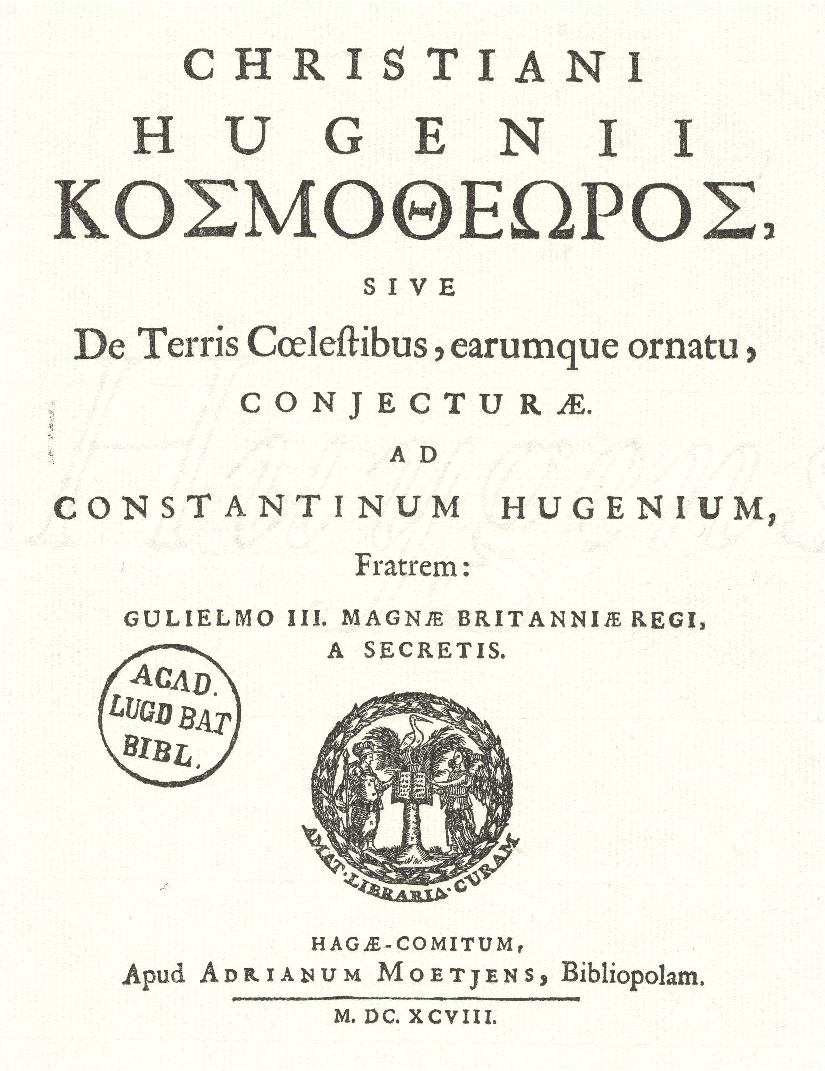
\includepdf{Images/ct_title_la.pdf}
\thispagestyle{empty}

\begin{titlepage}
	\begin{center}
\LARGE THE \\
\small \phantom{bla bla}
{\fontsize{42}{42} \fontspec{IM FELL English PRO}Celeſtial Worlds} \\
\small \phantom{bla bla}
\LARGE DISCOVER'D: \\
OR, \\
\fontsize{36}{36} \fontspec{IM FELL English PRO} \textsc{conjectures} \\
\fontsize{20}{36} \fontspec{IM FELL English PRO} Concerning the \\
\fontsize{36}{36} \fontspec{IM FELL English PRO} \textsc{inhabitants,} \\
\tiny \phantom{bla bla}
\fontsize{20}{24} \fontspec{IM FELL English PRO} \textsc{Plants} and \textsc{Productions} \\
\scriptsize 
\phantom{blabla}
\Large OF THE \\
\large \phantom{blabla}
{\fontsize{42}{36} \fontspec{Isabella}Worlds in the Planets} \\
\phantom{bla bla}
\hrule
\phantom{bla bla}
\Large
Written in Latin by \\
\emph{CHRISTIANUS HUYGENS}, \\
And inſcrib'd to his Brother \\
\emph{CONSTANTINE HUYGENS}, \\
Late Secretary to his Majeſty K. \emph{William} \\
\phantom{bla bla}
\hrule
\phantom{bla bla}
\textsc{\emph {LONDON}}, \\
Printed for \textsc{Timothy Childe} at the \\
White Hart at the Weſt-end of St. \\
\emph{Paul's} Church-yard. \, \, MDCXCVIII.
\end{center}
\end{titlepage}


\chapter{TO THE READER} % (fold)
\label{ſec:TO THE READER}
% manuaally inſert s's?
THIS Book was juſt finiſhed, and deſigned for the Preſs, when the Author,
to the great loſs of the Learned World, was ſeized by a Diſeaſe that brought
him to his Death. However he took care in his laſt Will of its Publication,
deſiring his Brother, to whom it was writ, to take that Trouble upon him.
But he was ſo taken up with Buſineſs and Removals, (as being Secretary in
Holland to the King of Great Britain) that be could find no time for it till
a year after the Death of the Author: When it ſo fell out, that the Printers
being ſomewhat tardy, and this Gentleman dying, the Book was left without
either Father or Guardian. Yet it now ventures into the Publick, in the ſame
method that it was writ by the Au[iv]thor, and with the ſame Inſcription to
his Brother, tho dead; in confidence that this laſt Piece of his will meet with
as kind a reception from the World as all the other Works of that Author
have. 'Tis true there are not every where Mathematical Demonſtrations; but
where they are wanting, you have probable and ingenious Conjectures, which
is the moſt that can be reaſonably expected in ſuch matters. What belongs
to, or has any thing to do with Aſtronomy, you will ſee demonſtrated, and
the reſt ingeniouſly and ſhrewdly gueſs'd at, from the affinity and relation
of the heavenly Bodies to the Earth. For your farther Satisfaction read on,
and farewel.
% ſection TO THE READER (end)

\chapter{THE PUBLISHER TO THE READER} 

\emph{ I Doubt not but I ſhall incur the Cenſures of learned Men for putting
this Book into Engliſh, becauſe, they'l ſay, it renders Philoſophy cheap and
vulgar, and, which is worſe, furniſhes a ſort of injudicious People with a
ſmattering of Notions, which being not able to make a proper uſe of, they
pervert to the Injury of Religion and Science. I confeſs the Allegation is
too true: but after Biſhop Wilkins, Dr. Burnet, Mr. Whiſton, and others, to
ſay nothing of the antient Philoſophers, who wrote in their own Tongues; I
ſay after theſe great Authors have treated on as learned and abſtruſe
Subjects in the ſame Language [vi] I hope their Example will be allowed a
ſufficient excuſe for printing this Book in Engliſh.  Concerning this
Edition I can ſay, that I have taken care to have the Cuts exactly done, and
have plac'd each Figure at the Page of the Book that refers to it, which I
take to be more convenient to the Reader than putting 'em all at the end.  I
have been careful to procure the beſt Paper; that I might in ſome meaſure
come up to the Beauty of the Latin Edition, tho this bear but half the Price
of it.  And l hope the Tranſlator has expreſs'd the Author's Senſe aright,
and has not committed Faults beyond what an ingenuous Reader can pardon.}

\tableofcontents
\mainmatter

\chapter{BOOK the Firſt}
\lettrine[lines=6, lraise=.26]{\fontspec[Scale=.78]{EB Garamond Initials} A}{ Man that is} of Copernicus's Opinion, that this Earth of ours is a Planet,
carry'd round and enlighten'd by the Sun, like the reſt of them, cannot but
[2] ſometimes have a fancy, that it's not improbable that the reſt of the
Planets have their Dreſs and Furniture, nay and their Inhabitants too as
well as this Earth of ours: Eſpecially if he conſiders the later Diſcoveries
made ſince Copernicus's time of the Attendents of Jupiter and Saturn, and
the Champain and hilly Countrys in the Moon, which are an Argument
of a relation and kin between our Earth and them, as well as a proof of
the Truth of that Syſtem. This has often been our talk, I remember, good
Brother, over a large Teleſcope, when we have been viewing thoſe Bodies,
a ſtudy that your continual buſineſs and abſence have interrupted for this
many years, But we were always apt to conclude, that 'twas in vain to
enquire after what Nature had been pleaſed to do there, ſeeing there was
no likelihood of ever coming to an end of the Enquiry. Nor could I ever find
that any Philoſophers, thoſe bold Heros, either antient or modern, ventur'd
ſo far. At the very birth of Aſtronomy, when the Earth was firſt aſſerted
to [3] be Spherical, and to be ſurrounded with Air, even then there were
ſome men ſo bold as to affirm, that there were an innumerable company of
Worlds in the Stars.


\section{Some have already talk'd of the Inhabitants of the
Planets, but went no farther}

Bur later Authors, ſuch as Cardinal Cuſanus, Brunus, Kepler (and if we may
believe him, Tycho was of that opinion too) have furniſh'd the Planets with
Inhabitants. Nay, Cuſanus and Brunus have allow'd the Sun and fixed Stars
theirs too. But this was the utmoſt of their boldneſs; nor has the ingenious
French Author of the Dialogues about the Plurality of Worlds carry'd the
buſineſs any farther. Only ſome of them have coined ſome pretty Fairy
Stories of the Men in the Moon, juſt as probable as Lucian's true Hiſtory;
among which I muſt count Kepler's, which he has diverted us with in his
Aſtronomical Dream. But a while ago thinking ſomewhat ſeriouſly of this
matter (not that I count my ſelf quicker ſighted than thoſe great Men, but
that I had the happineſs to live after moſt of them) methoughts the enquiry
was not ſo impracticable, nor the way ſo [4] ſtopt up with Difficulties, but
that there was very good room left for probable Conjectures. As they came
into my head, I clapt them down into common places, and ſhall now try to
digeſt them into ſome tolerable Method for your better conception of them,
and add ſomewhat of the Sun and Fixt Stars, and the Extent of that Univerſe
of which our Earth is but an inconſiderable point. I know you have ſuch an
eſteem and reverence for any thing that belongs to Heaven, that I perſwade
my ſelf you will read what I have written without pain: I'm ſure I writ it
with a great deal of pleaſure; but as often before, ſo now, I find the
ſaying of Archytas true, even to the Letter, That tho a Man were admitted
into Heaven to view the wonderful Fabrick of the World, and the Beauty of
the Stars, yet what would otherwiſe be Rapture and Extaſie, would be but a
melancholy Amazement if he had not a Friend to communicate it to. I could
wiſh indeed that all the World might not be my Judges, but that I might
chuſe my Readers, Men like you, not [5] ignorant in Aſtronomy and true
Philoſophy; for with ſuch I might promiſe my ſelf a favourable hearing, and
not need to make an Apology for daring to vent any thing new to the World.
But becauſe I am aware what other hands it's likely to fall into, and what a
dreadful Sentence I may expect from thoſe whoſe Ignorance or Zeal is too
great, it may be worth the while to guard my ſelf beforehand againſt the
Aſſaults of thoſe ſort of People.


\section{The Objections of ignorant Cavillers prevented}

There's one ſort who knowing nothing of Geometry or Mathematicks, will laugh
at it as a whimſical and ridiculous undertaking. It's mere Conjuration to
them to talk of meaſuring the Diſtance or Magnitude of the Stars: And for
the Motion of the Earth, they count it, if not a falſe, at leaſt a
precarious Opinion; and no wonder then if they take what's built upon ſuch a
ſlippery Foundation for the Dreams of a fanciful Head and a diſtemper'd
Brain.  What ſhould we anſwer to theſe Men, but that their Ignorance is the
cauſe of their Diſlike, and that if they had more Senſe they [6] would have
fewer Scruples? But few people having had an opportunity of proſecuting
theſe Studies, either for want of Parts, Learning, or Leiſure, we cannot
blame their Ignorance; and if they reſolve to find fault with us for
ſpending time in ſuch matters, becauſe they do not underſtand the uſe of
them, we muſt appeal to properer Judges.


\section{Theſe Conjectures do not contradict the holy Scriptures}

The other ſort, when they hear us talk of new Lands, and Animals endued with
as much Reaſon as themſelves will be ready to fly out into religious
Exclamations, that we ſet up Conjectures againſt the Word of God, and broach
Opinions directly oppoſite to Holy Writ. For we do not there read one word
of the Production of ſuch Creatures, no not ſo much as of their Exiſtence;
nay rather we read the quite contrary. For, That only mentions this Earth
with its Animals and Plants, and Man the Lord of them; but as for Worlds in
the Sky, 'tis wholly ſilent. Either theſe Men reſolve not to underſtand, or
they are very ignorant; For they have [7] been anſwer'd ſo often, that I am
almoſt aſham'd to repeat it: That it's evident God had no deſign to make a
particular Enumeration in the Holy Scriptures, of all the Works of his
Creation. When therefore it is plain that under the general name of Stars or
Earth are comprehended all the Heavenly Bodies, even the little Gentlemen
round Jupiter and Saturn, why muſt all that multitude of Beings which the
Almighty Creator has been pleaſed to place upon them, be excluded the
Privilege, and not ſuffer'd to have a ſhare in the Expreſſion?  And theſe
Men themſelves can't but know in what ſenſe it is that all things are ſaid
to be made for the uſe of Man, not certainly for us to ſtare or peep through a
Teleſcope at; for that's little better than nonſenſe. Since then the
greateſt part of God's Creation, that innumerable multitude of Stars, is
plac'd out of the reach of any man's Eye; and many of them, it's likely, of
the beſt Glaſſes, ſo that they don't ſeem to belong to us; is it ſuch an
unreaſonable Opinion, that there are [8] ſome reaſonable Creatures who ſee
and admire thoſe glorious Bodies at a nearer diſtance?


\section{This Enquiry not overcurious}

But perhaps they'll ſay, it does not become us to be ſo curious and
inquiſitive in theſe things which the Supreme Creator ſeems to have kept for
his own knowlege: For ſince he has not been pleaſed to make any farther
Diſcovery or Revelation of them, it ſeems little better than preſumption to
make any inquiry into that which he has thought fit to hide. But theſe
Gentlemen muſt be told, that they take too much upon themſelves when they
pretend to appoint how far and no farther Men ſhall go in their Searches,
and to ſet bounds to other Mens Induſtry; juſt as if they had been of the
Privy Council of Heaven: as if they knew the Marks that God has plac'd to
Knowlege: or as if Men were able to paſs thoſe Marks. If our Forefathers had
been at this rate ſcrupulous, we might have been ignorant ſtill of the
Magnitude and Figure of the Earth, or of ſuch a place as America. The Moon
might have [9] ſhone with her own Light for all us, and we might have ſtood
up to the ears in Water, like the Indians at every Eclipſe: and a hundred
other things brought to light by the late Diſcoveries in Aſtronomy had ſtill
been unknown to us. For what can a Man imagine more abſtruſe, or leſs likely
to be known, than what is now as clear as the Sun? That vigorous Induſtry,
and that piercing Wit were given Men to make advances in the ſearch of
Nature, and there's no reaſon to put any ſtop to ſuch Enquiries. I muſt
acknowlege ſtill that what I here intend to treat of is not of that nature
as to admit of a certain knowlege; I can't pretend to aſſert any thing as
poſitively true (for that would be madneſs) but only to advance a probable
gueſs, the truth of which every one is at his own liberty to examine. If any
one therefore ſhall gravely tell me, that I have ſpent my time idly in a
vain and fruitleſs enquiry after what by my own acknowlegement I can never
come to be ſure of; the anſwer is, that at this rate he would put down all
[10] Natural Philoſophy as far as it concerns it ſelf in ſearching into the
Nature of things:


\section{Conjectures not uſeleſs, becauſe not certain}

In ſuch noble and ſublime Studies as theſe, 'tis a Glory to arrive at
Probability, and the ſearch it ſelf rewards the pains. But there are many
degrees of Probable, ſome nearer Truth than others, in the determining of
which lies the chief exerciſe of our Judgment.


\section{Theſe Studies uſeful to Religion}

But beſides the Nobleneſs and Pleaſure of the Studies, may not we be ſo bold
as to ſay, they are no ſmall help to the advancement of Wiſdom and Morality?
ſo far are they from being of no uſe at all. For here we may mount from this
dull Earth, and viewing it from on high, conſider whether Nature has laid
out all her coſt and finery upon this ſmall ſpeck of Dirt.  So, like
Travellers into other diſtant Countrys, we ſhall be better able to judg of
what's done at home, know how to make a true eſtimate of, and ſet its own
value upon every thing. We ſhall be leſs apt to admire what this World calls
great, ſhall nobly deſpiſe thoſe Trifles the generality of Men ſet their
Affections [11] on, when we know that there are a multitude of ſuch Earths
inhabited and adorned as well as our own. And we ſhall worſhip and reverence
that God the Maker of all theſe things; we ſhall admire and adore his
Providence and wonderful Wiſdom which is diſplayed and manifeſted all over
the Univerſe, to the confuſion of thoſe who would have the Earth and all
things formed by the ſhuffling Concourſe of Atoms, or to be without
beginning. But to come to our purpoſe.


\section{Copernicus's Syſtem explain'd}

And now becauſe the chief Argument for the proof of what we intend will be
taken from the diſpoſition of the Planets, among which without doubt the
Earth muſt be counted in the Copernican Syſtem, I ſhall here firſt of all
draw two Figures. 

\begin{center}
	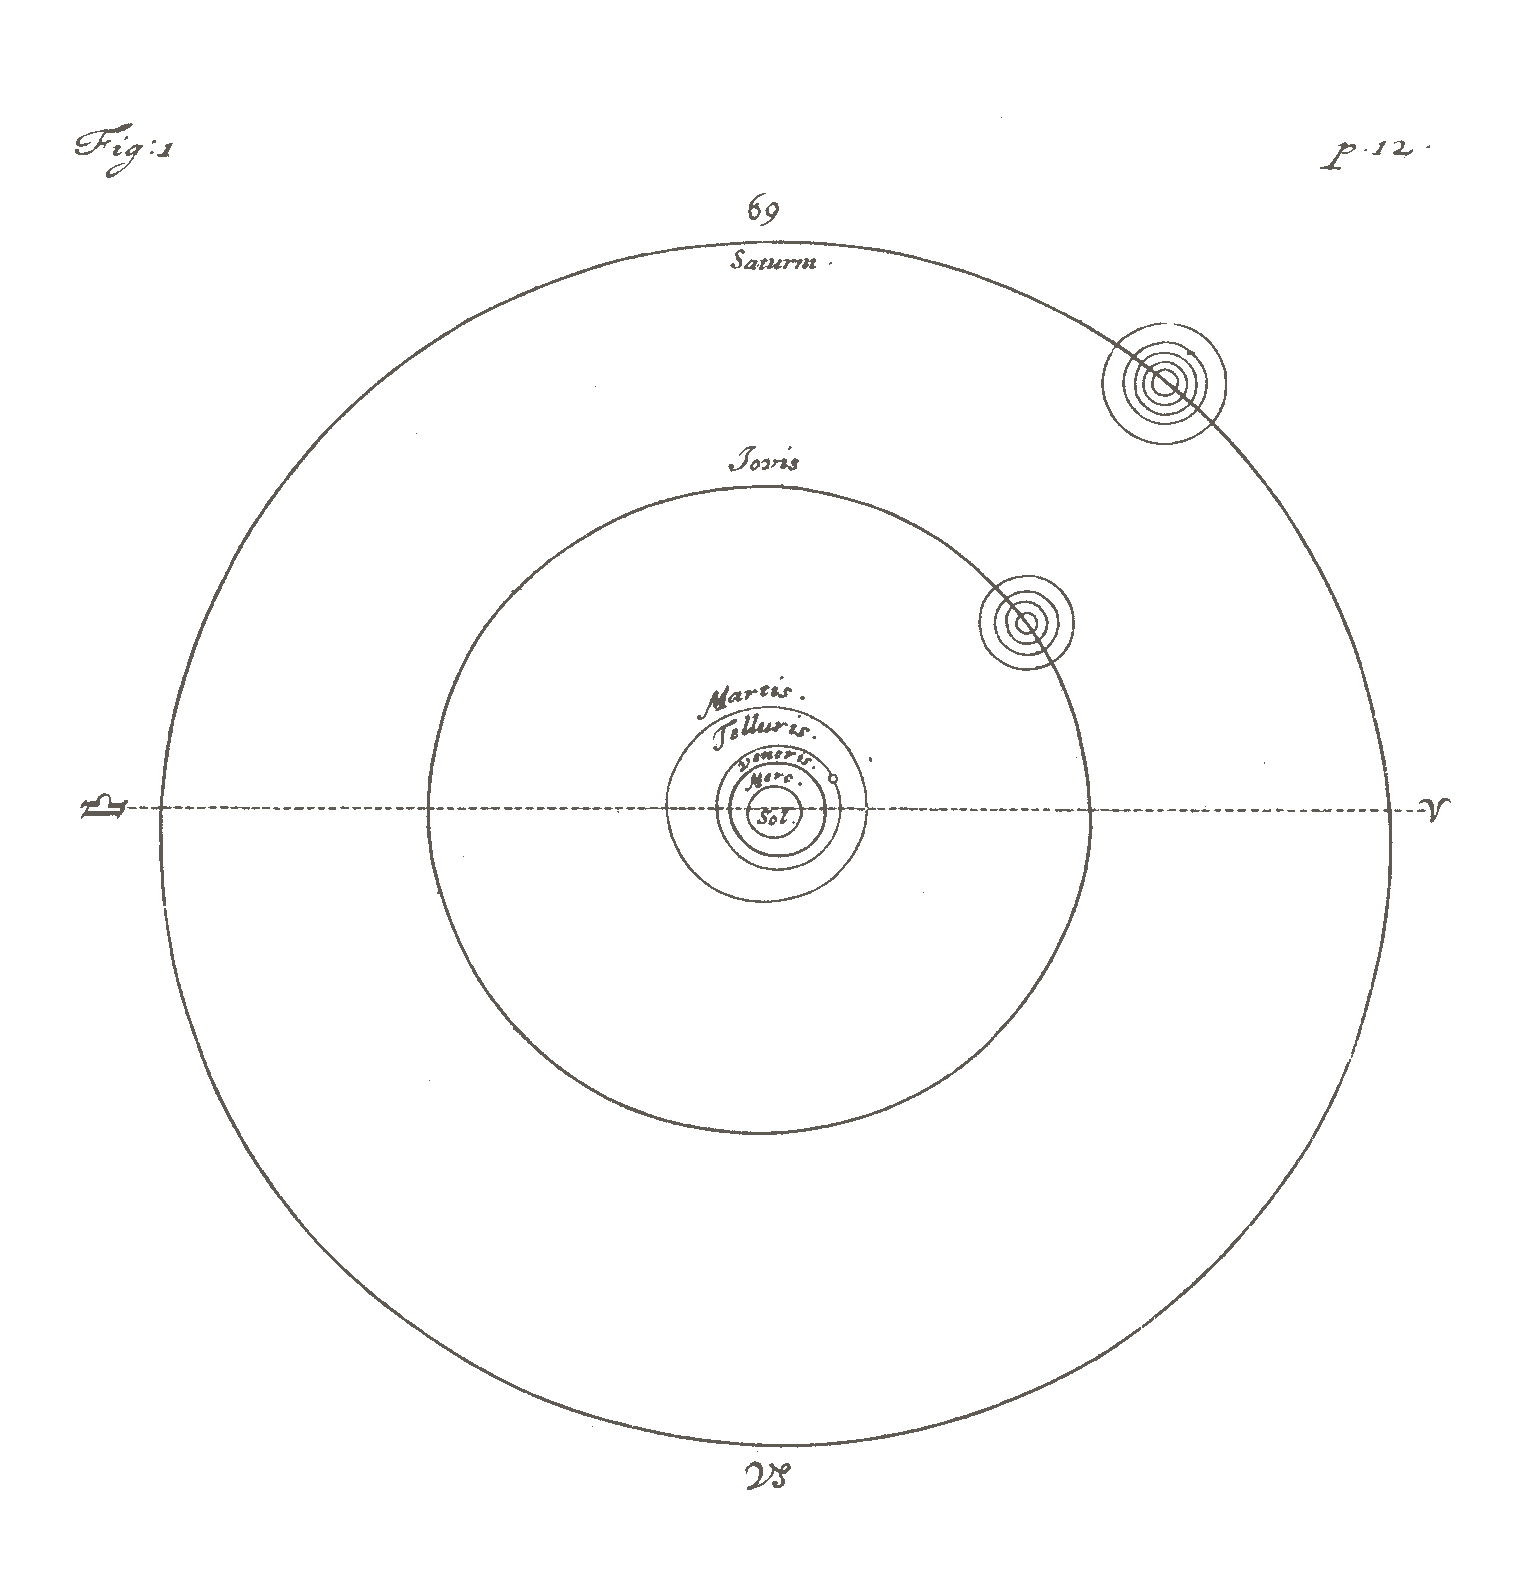
\includegraphics[width=.90 \textwidth]{Images/ct_1_en.jpg}
\end{center}


The firſt is a Deſcription of the Orbs the Planets move
in, in that order that they are placed round the Sun, drawn as near as can
be in their true Proportions, like what you have ſeen in my Clock at home.
The ſecond ſhows the Proportions of their Magnitudes in reſpect of one
another and of the [12] Sun, which you know is upon that ſame Clock of mine
too. In the firſt the middle Point or Center is the Place of the Sun, round
which, in an order that everyone knows, are the Orbits of Mercury, Venus,
the Earth with that of the Moon about it; then thoſe of Mars, Jupiter and
Saturn: and about the two laſt the ſmall Circles that their Attendents march
in: about Jupiter four, and about Saturn five. Which Circles as well as that
of the Moon are drawn larger than their true Proportion would admit,
otherwiſe they could not have been ſeen. You may eaſily apprehend the
Vaſtneſs of theſe Orbits by this, that the diſtance of the Earth from the
Sun is ten or twelve thouſand of the Earth's Diameters. Almoſt all theſe
Circles are in the ſame Plane, declining very little from that in which the
Earth moves, call'd the Plane of the Ecliptick. This Plane is cut obliquely
by the Axis upon which the Earth turns it ſelf round in 24 hours, whence
ariſe the Succeſſions of Day and Night: The Axis of the Earth always
keep[13]ing the ſame Inclination to the Ecliptick (except a ſmall change
beſt known to Aſtronomers) while the Earth it ſelf is carry'd in its yearly
Courſe round the Sun, cauſes the regular Order of the Seaſons of the Year:
as you may ſee in all Aſtronomers Books.  Out of which I ſhall tranſcribe
hither the Periods of the Revolutions of the Planets, viz. Saturn moves
round the Sun in 29 Years, 174 Days, and 5 Hours: Jupiter finiſhes his
Courſe in 11 Years, 317 Days, and 15 Hours: Mars his in about 687 Days. Our
Year is 365 Days 6 Hours: Venus's 224 Days 18 Hours: and Mercury's 88 Days.
This is the now commonly receiv'd Syſtem, invented by Copernicus, and very
agreeable to that frugal Simplicity Nature ſhows in all her Works.


\section{Arguments for the truth of it}

If any one is reſolved to find fault with it, let him firſt be ſure he
underſtands it. Let him firſt ſee in the Books of Aſtronomers with how much
greater eaſe and plainneſs all the Motions of the Stars, and Appearances in
the Heavens are explained and demonſtrated in this than either in [14] that
of Ptolemy or Tycho. Let him conſider that Diſcovery of Kepler, that the
diſtances of the Planets from the Sun, as well of the Earth as the reſt; are
in a fixt certain proportion to the times they ſpend in their Revolutions.
Which Proportion it's ſince obſerved that their Satellites keep round
Jupiter and Saturn. Let him examine what a contradictory Motion they are
fain to invent for the ſolution of the Polar Star's changing its diſtance
from the Pole. For that Star in the end of the Little Bear's Tail which now
deſcribes ſo ſmall a Circle round the Pole, that it is not above two Degrees
and twenty Minutes, was obſerved about 1820 Years ago, in the time of
Hipparchus, to be above 12: and will within a few ages more be forty five
Degrees diſtant from it: and after 25000 years more will return to the ſame
place it is now in. Now if with them we allow the Heavens to be turned upon
their own Axis, at this rate they muſt have a new Axis every day: a thing
moſt abominably abſurd, and repugnant to the nature of all motion.
Where[15]as nothing is eaſier with Copernicus than to give us ſatisfaction
in this matter. Then he may impartially weigh thoſe Anſwers that Galileus,
Gaſſendus, Kepler, and others have given to all Objections propoſed, which
have ſo ſatisfied all Scruples, that generally all Aſtronomers now adays are
brought over to our ſide, and allow the Earth its Motion and Place among the
Planets. If he cannot be ſatisfied with all this, he is either one whoſe
Dulneſs can't comprehend it, or who has his Faith at another man's diſpoſal,
and ſo for fear of Galileo's fate dare not own it.

\begin{center}
	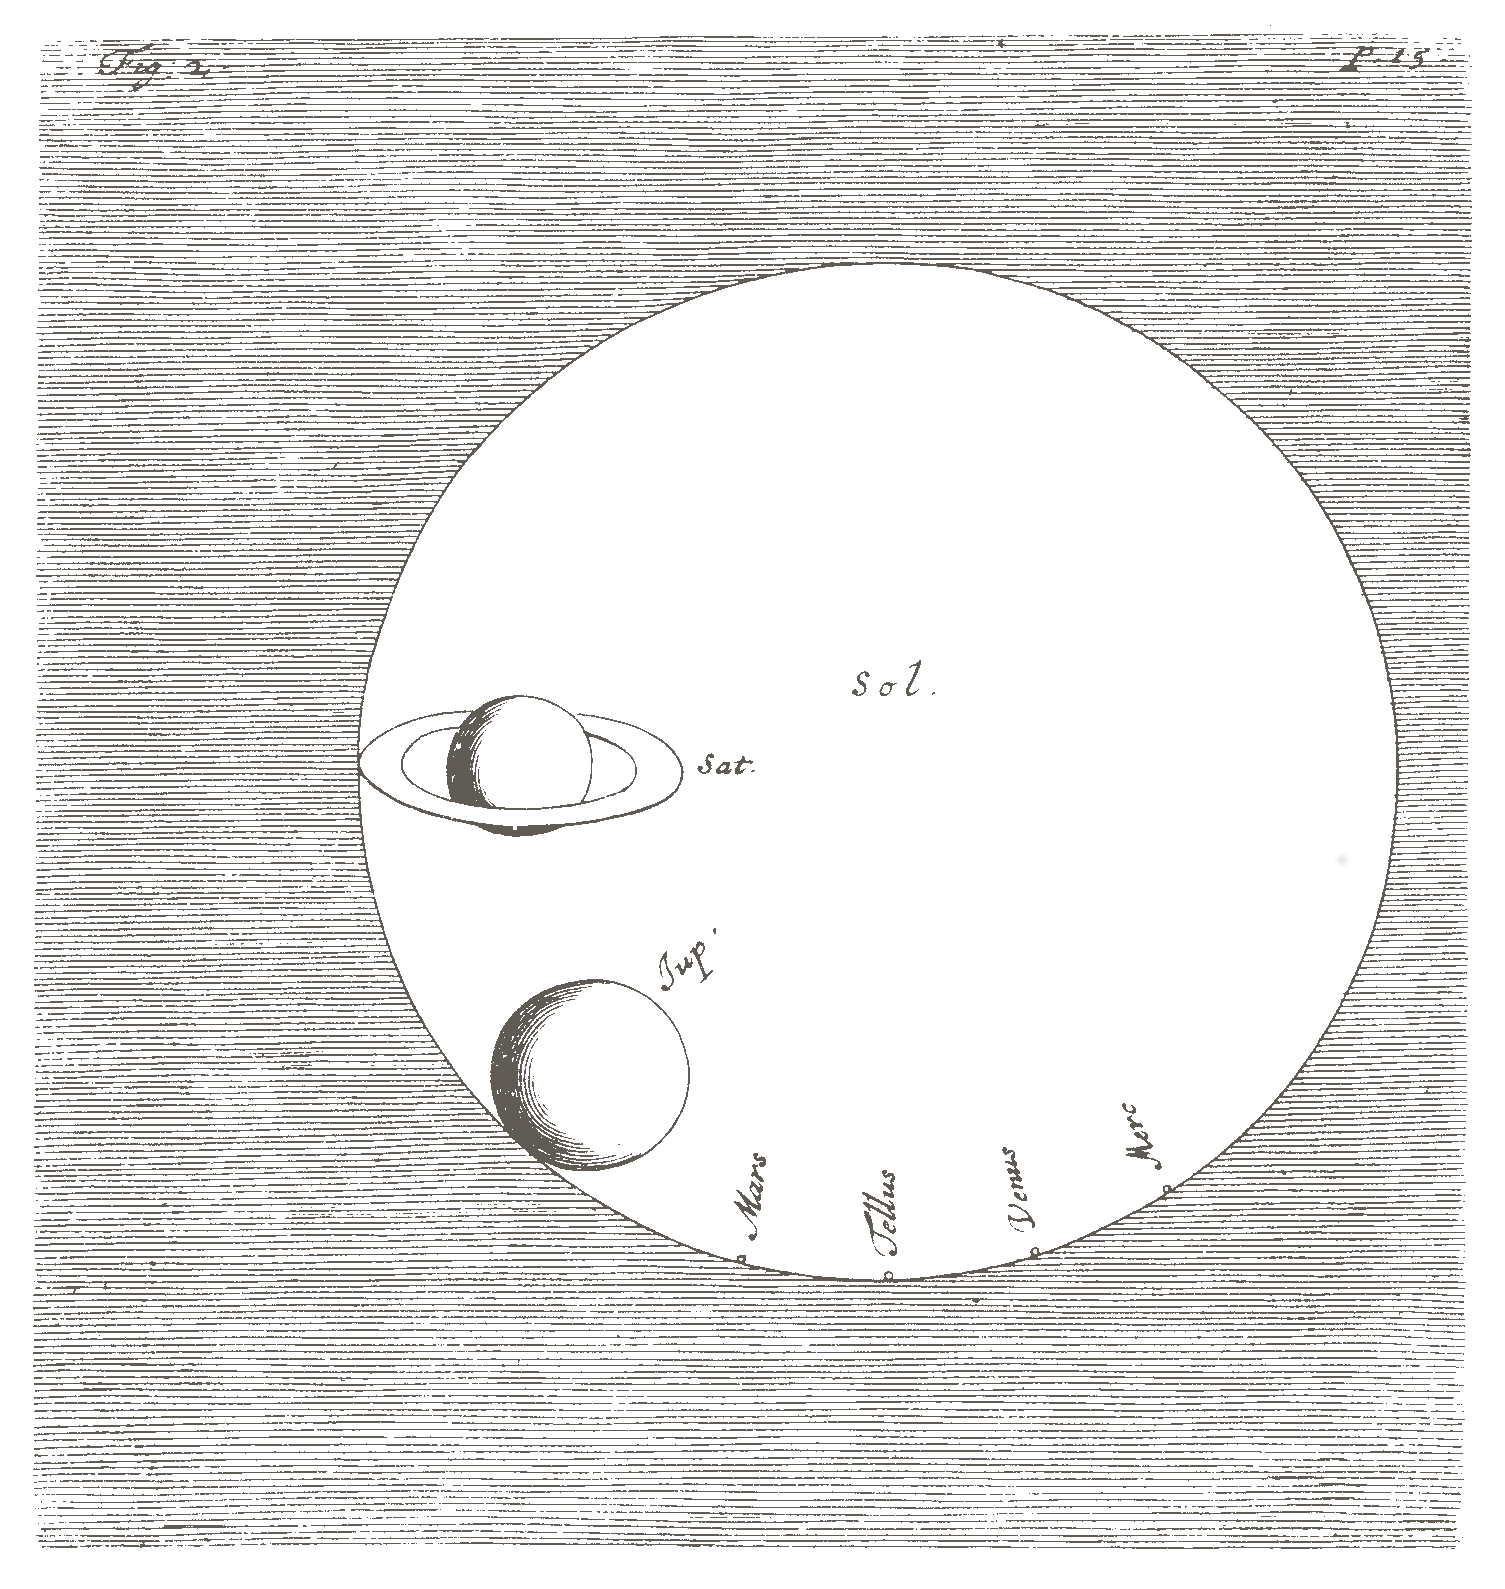
\includegraphics[width=.90 \textwidth]{Images/ct_2_en.jpg}
\end{center}


\section{The Proportion of the Magnitude of the Planets, in
reſpect of one another, and the Sun}

In the other Figure you have the Globes of the Planets, and of the Sun,
repreſented to your eyes as plac'd near one another. Where I have obſerv'd
the ſame Proportion of their Diameters to that of the Sun, that I publiſh'd
to the World in my Book of the Appearances of Saturn: namely, the Diameter
of the Ring round Saturn is to that of the Sun as 11 is to 37; that of
Saturn himſelf about as 5 to 37; that of Jupiter as 2 to 11; that [16] of
Mars as 1 to 166; of the Earth as 1 to 111; and of Venus as 1 to 84: to
which I ſhall now add that of Mercury obſerv'd by Hevelius in the Year 1661,
but calculated by my ſelf, and found to be as 1 to 290.


\section{The Lamellæ more convenient than Micrometers}

If you would know the way that we came to this knowledg of their Magnitudes,
by knowing the Proportion of their Diſtances from the Sun, and the meaſure of
their Diameters, you may find it in the Book beforementioned: and I cannot yet
ſee any reaſon to make an alteration in thoſe I then ſettled, altho I will not
ſay they are without their faults.  For I can't yet be of their mind, who
think the uſe of micrometers, as they call them, is beyond that of our Plates,
but muſt ſtill think that thoſe thin Plates or Rods of which I there taught
the uſe, not to detract from the due praiſes of ſo uſeful an Invention, are
more convenient than the Micrometers.


\section{The Earth juſtly liken'd to the Planets, and the
Planets to it}

In this Proportion of the Planets it is worth while to take notice of the
prodigious Magnitude of the Sun in compariſon with the four innermoſt, [17]
which are far leſs than Jupiter and Saturn. And ‘tis remarkable, that the
Bodies of the Planets do not increaſe together with their diſtances from the
Sun, but that Venus is much bigger than Mars.  Having thus explain'd the two
Schemes, there's no body I ſuppoſe but, ſees, that in the firſt the Earth is
made to be of the ſame ſort with the reſt of the Planets. For the very
Poſition of the Circles ſhows it. And that the other Planets are round like
it, and like it receive all the Light they have from the Sun, there's no
room (ſince the Diſcoveries made by Teleſcopes) to doubt, Another thing they
are like it in is, that they are moved round their own Axis; for ſince 'tis
certain that Jupiter and Saturn are, who can doubt it of the others? Again,
as the Earth has its Moon moving round it, ſo Jupiter and Saturn have
theirs. Now ſince in ſo many things they thus agree, what can be more
probable than that in others they agree too; and that the other Planets are
as beautiful and as well ſtock'd with [18] Inhabitants as the Earth? or what
ſhadow of Reaſon can there be why they ſhould not?  If anyone ſhould be at
the diſſection of a Dog, and be: there ſhewn the Intrails, the Heart,
Stomach, Liver, Lungs and Guts, all the Veins, Arteries and Nerves; could
ſuch a Man reaſonably doubt whether there were the ſame Contexture and
Variety of Parts in a Bullock, Hog, or any other Beaſt, tho he had never
chanc'd to ſee the like opening of them? I don't believe he would. Or were
we thorowly ſatisfy'd in the Nature of one of the Moons round Jupiter,
ſhould not we ſtraight conclude the ſame of the reſt of them?  So if we
could be aſſur'd in but one Comet, what it was that is the cauſe of that
ſtrange appearance, ſhould we not make that a Standard to judg of all others
by?


\section{Arguments from their Similitude of no ſmall weight}

'Tis therefore an Argument of no ſmall weight that is fetch'd from Relation
and Likeneſs; and to reaſon from what we ſee and are ſure of, to what we
cannot, is no falſe Logick. This muſt be our Method in this Treatiſe, [19]
wherein from the Nature and Circumſtances of that Planet which we ſee
before our eyes, we may gueſs at thoſe that are farther diſtant from us.


\section{The Planets are ſolid, and not without Gravity}

And; Firſt, 'tis more than probable that the Bodies of the Planets are ſolid
like that of our Earth, and that they don't want what we call Gravity, that
Virtue, which like a Loadſtone attracts whatſoever is near the Body to its
Center. And that they have ſuch a quality, their very Figure is a proof; for
their Roundneſs proceeds only from an equal preſſure of all their Parts
tending to the ſame Center. Nay more, we are ſo skilful now adays, as to be
able to tell how much more or leſs the Gravitation in Jupiter or Saturn is
than here; of which Diſcovery and its Author you may read my Eſſay of the
Cauſes of Gravitation.


\section{Have Animals and Plants}

But now to carry the ſearch farther, let us ſee by what ſteps we muſt riſe
to the attaining ſome knowlege in the more private Secrets concerning the
State and Furniture of theſe new Earths. And, firſt, how likely is it [20]
that they may be ſtock'd with Plants and Animals as well as we? I ſuppoſe no
body will deny but that there's ſomewhat more of Contrivance, ſomewhat
more of Miracle in the production and growth of Plants and Animals, than in
lifeleſs heaps of inanimate Bodies, be they never ſo much larger; as
Mountains, Rocks, or Seas are. For the finger of God, and the Wiſdom of
Divine Providence, is in them much more clearly manifeſted than in the
other. One of Democritus's or Cartes's Scholars may venture perhaps to give
ſome tolerable Explication of the appearances in Heaven and Earth, allow him
but his Atoms and Motion; but when he comes to Plants and Animals, he'll
find himſelf non-plus'd, and give you no likely account of their Production.
For every thing in them is ſo exactly adapted to ſome deſign, every part of
them ſo fitted to its proper life, that they manifeſt an Infinite Wiſdom,
and exquiſite Knowlege in the Laws of Nature and Geometry, as, to omit thoſe
Wonders in Generation, we ſhall by and by ſhow; and [21] make it an
abſurdity even to think of their being thus haply jumbled together by a
chance Motion of I don't know what little Particles. Now ſhould we allow the
Planets nothing but vaſt Deſerts, lifeleſs and inanimate Stocks and Stones,
and deprive them of all thoſe Creatures that more plainly ſpeak their Divine
Architect, we ſhould ſink them below the Earth in Beauty and Dignity; a
thing that no Reaſon will permit, as I ſaid before.  Well then, now we have
gain'd the Point for them, and the Planets may be allow'd ſome Bodys capable
of moving themſelves, not at all inferior to ours, (for why ſhould they?)
and theſe are Animals. Now for fear of ſtarving there poor Creatures, we
muſt have Plants you know. And ſo the other Point is gain'd. And as for
their Growth and Nouriſhment, 'tis no doubt the ſame with ours, ſeeing they
have the ſame Sun to warm and enliven them as ours have.


\section{Not to be imagin'd too unlike ours}

But perhaps ſome body may ſay, we conclude too faſt. They will not deny
indeed but that there may be [22] Plants and Animals on the Surface of the
Planets, that deſerve as well to be provided for by their Creator as ours
do: but why muſt they be of the ſame nature with ours? Nature ſeems to court
variety in her Works, and may have made them widely different from ours
either in their matter or manner of Growth, in their outward Shape, or their
inward Contexture; ſhe may have made them ſuch as neither our Underſtanding
nor Imagination can conceive. That's the thing we ſhall now examin, and
whether it be not more likely that ſhe has not obſerv'd ſuch a variety as
they talk of. Nature ſeems moſt commonly, and in moſt of her Works, to
affect Variety, 'tis true; But they ſhould conſider 'tis not the buſineſs of a
man to pretend to ſettle how great this Difference and Variety muſt be. Nor
does it follow, becauſe it may be Infinite, and out of our comprehenſion and
reach, that therefore things in reality are ſo. For ſuppoſe God ſhould have
pleaſed to have made all things there juſt as he has here, the Inhabitants
of thoſe Places (if there [23] are any ſuch ſtrange things) would admire his
Wiſdom and Contrivance no leſs than if they were widely different; ſeeing
they can't come to know what's done in the other Planets.  Who doubts but
that God, if he had pleaſed, might have made the Animals in America and
other diſtant Countries nothing like ours? (and Nature you know affects
Variety) yet we ſee he has not done it. They have indeed ſome difference in
their ſhape, and 'tis fit they ſhould, to diſtinguiſh the Plants and Animals
of thoſe Countries from ours, who live on this ſide the Earth; but even in
this variety there is an Agreement, an exact Correſpondence in figure and
ſhape, the ſame ways of Growth, and new Productions, and of continuing their
own kind. Their Animals have Feet and Wings like ours, and like ours have
Heart, Lungs, Guts, and the Parts ſerving to Generation; whereas all theſe
things, as well with them as us, might, if it had ſo pleaſed Infinite
Wiſdom, have been order'd a very different way. 'Tis plain then that
Na[24]ture has not exhibited that Variety in her Works that ſhe could, and
therefore we muſt not allow that weight to this Argument, as upon the
account of it to make every thing in the Planets quite different from what
is here. 'Tis more probable that all the difference there is between us and
them, ſprings from the greater or leſs diſtance and influence from that
Fountain of Heat and Life the Sun; which will cauſe a difference not ſo much
in their Form and Shape, as in their Matter and Contexture.


\section{Planets have Water}

And as for the matter whereof the Plants and Animals there conſiſt, tho it
is impoſſible ever to come to the knowlege of its Nature, yet this we may
venture to aſſert (there being ſcarce any doubt of it) that their Growth and
Nouriſhment proceeds from ſome liquid Principle. Far all Philoſophers agree
that there can be no other way of Nutrition; ſome of the chief among them
having made Water to be the Original of all things: Far whatſoever's dry and
without moiſture, is without motion too; and [25] without motion it's
impoſſible there ſhould be any increaſe. But the parts of a Liquid being in
continual motion one with another, and inſinuating and twiſting themſelves
into the ſmalleſt Places, are thereby very proper and apt to add not
themſelves only, but whatſoever elſe they may bring along with them to the
increaſe and growth of Bodies. Thus we ſee that by the means of Water the
Plants grow, bloſſom, and bear Fruit; and by the addition of that only,
Stones grow together out of Sand. And there's no doubt but that Metals,
Cryſtals, and Jewels, have the ſame method of Production: Tho in them there
has been no opportunity to make the ſame obſervation, as well by reaſon of
their ſlow advances, as that they are commonly found far from the Places of
their Generation; thrown up I ſuppoſe by ſome Earthquakes or Convulſions.
That the Planets are not without Water, is made not improbable by the late
Obſervations: For about Jupiter are obſerv'd ſome ſpots of a darker hue than
the reſt of his Body, [26] which by their continual change ſhow themſelves
to be Clouds: For the ſpots of Jupiter which belong to him, and never remove
from him, are quite different from theſe, being ſometimes for a long time
not to be ſeen for theſe Clouds; and again, when there diſappear, ſhowing
themſelves. And at the going off of theſe Clouds, ſome ſpots have been taken
notice of in him, much brighter than the reſt of his Body, which remain'd
but a little while, and then were hid from our ſight. Theſe Monſieur Caſſini
thinks are only the Reflection from the Snow that covers the tops of the
Hills in Jupiter: but I ſhould rather think that it is only the colour of
the Earth, which chances to be free from thoſe Clouds that commonly darken
it.  Mars too is found not to be without his dark ſpots, by means of which
he has been obſerv'd to turn round his own Axis in 24 hours and 40 minutes;
the length of his day: but whether he has Clouds or no, we have not had the
ſame opportunity of obſerving as in Jupiter, as well becauſe even when [27]
he is neareſt the Earth, he appears to us much leſs than Jupiter, as that
his Light not coming ſo long a Journey, is ſo brisk as to be an Impediment
to exact Obſervations: And this Reaſon is as much ſtronger in Venus as its
Light is. But ſince 'tis certain that the Earth and Jupiter have their Water
and Clouds, there is no reaſon why the other Planets ſhould be without them.


\section{But not juſt like ours}

I can't ſay that they are exactly of the ſame nature with our Water; but
that they ſhould be liquid their uſe requires, as their beauty does that they
ſhould be clear. For this Water of ours, in Jupiter or Saturn, would be
frozen up inſtantly by reaſon of the vaſt diſtance of the Sun. Every Planet
therefore muſt have its Waters of ſuch a temper, as to be proportion'd to
its heat: Jupiter's and Saturn's muſt be of ſuch a nature as not to be liable
to Froſt; and Venus's and Mercury's of ſuch, as not to be eaſily evaporated
by the Sun. But in all of them, for a continual ſupply of Moiſture, whatever
Water is drawn up by the Heat of the Sun into Vapors, muſt neceſſa[28]rily
return back again thither. And this it cannot do but in drops, which are
cauſed as well there as with us, by their aſcending into a higher and colder
Region of the Air, out of that which, by reaſon of the Reflection of the Rays
of the Sun from the Earth, is warmer and more temperate.


\section{Plants grow and are nouriſh'd there as they are here}

Here then we have found in there new Worlds Fields warm'd by the kindly Heat
of the Sun, and water'd with fruitful Dews and Showers: That there muſt be
Plants in them as well for Ornament as Uſe, we have ſhewn juſt now. And what
Nouriſhment, what manner of Growth ſhall we allow them?  Why, I think there
can be no better, nay no other, than what we here experience; by having
their Roots faſtned into the Earth, and imbibing its nouriſhing Juices by
their tender Fibres. And leſt they ſhould be only like ſo many bare Heaths,
with nothing but creeping Shrubs and Buſhes, we'll e'en ſend them ſome
nobler and loftier Plants, Trees, or ſomewhat like them: Theſe being the
greateſt, and, except Waters, the only [29] Ornament that Nature has
beſtow'd upon the Earth. For not to ſpeak of thoſe many uſes that are made
of their Wood, there's no one that is ignorant either of their Beauty or
Pleaſantneſs. Now what way can anyone imagine for a continual Production and
Succeſſion of theſe Plants, but their bearing Seed? A Method ſo excellent
that it's the only one that Nature has here made uſe of, and ſo wonderful,
that it ſeems to be deſign'd not far this Earth alone. In fine, there's the
ſame reaſon to think that this Method is obſerv'd in thoſe diſtant
Countries, as there was of its being follow'd in the remote Quarters of this
ſame Earth.


\section{The ſame true of their Animals}

'Tis much the ſame in Animals as 'tis in Plants, as to their manner of
Nouriſhment, and Propagation of their kind. For ſince all the living Creatures
of this Earth, whether Beaſts, Birds, Fiſhes, Worms, or Inſects, univerſally
and inviolably follow the ſame conſtant and fixt Inſtitution of Nature; all
feed on Herbs, or Fruits, or the Fleſh of other Animals that fed [30] on them:
ſince all Generation is perform'd by the impregnating of the Eggs, and the
Copulation of Male and Female: Why may not the ſame rule be obſerv'd in the
Planetary Worlds? For't is certain that the Herbs and Animals that are there
would be loſt, their whole Species deſtroy'd without ſome daily new
Productions: except there be no ſuch thing there as Misfortune or Accident:
except the Plants are not like other humid Bodies, but can bear Heat, Froſt
and Age, without being dry'd up, kill'd, or decay'd: except the Animals have
Bodies as hard and durable as Marble; which I think are groſs Abſurdities. If
we ſhould invent ſome new way for their coming into the World, and make them
drop like Soland Geeſe from Trees, how ridiculous would this be to any one
that conſiders the vaſt difference between Wood and Fleſh? Or ſuppoſe we
ſhould have new ones made every day out of ſome ſuch fruitful Mud as that of
Nile, who does not ſee how contrary this is to all that's reaſonable? And that
'tis much more agreeable to [31] the Wiſdom of God, once for all to create of
all ſorts of Animals, and diſtribute them all over the Earth in ſuch a
wonderful and inconceivable way as he has, than to be continually obliged to
new Productions out of the Earth?  And what miſerable, what helpleſs Creatures
muſt theſe be, when there's no one that by his duty will be obliged, or by
that ſtrange natural fondneſs, which God has wiſely made a neceſſary argument
for all Animals to take care of their own, will be moved to aſſiſt, nurſe or
educate them?  As for what I have ſaid concerning their Propagation, I cannot
be ſo poſitive; but the other thing, namely, that they have Plants and
Animals, I think I have fully proved. And by the ſame Argument, of their not
being inferiour to our Earth, they muſt have as great a variety of both as we
have. What this is, will be beſt known to him that conſiders the different
ways our Animals make uſe of in moving from one place to another. Which may be
reduc'd, I think, to theſe; ei[32]ther that they walk upon two feet or four;
or like Inſects, upon ſix, nay ſometimes hundreds; or that they fly in the Air
bearing up, and wonderfully ſteering themſelves with their Wings; or creep
upon the Ground without feet; or by a violent Spring in their Bodies, or
paddling with their feet, cut themſelves a way in the Waters.  I don't
believe, nor can I conceive, that there ſhould be any other way than theſe
mention'd. The Animals then in the Planets muſt make uſe of one or more of
theſe, like our amphibious Birds, which can ſwim in Water as well as walk on
Land, or fly in the Air; or like our Crocodiles and Sea-Horſes, muſt be
Mongrels, between Land and Water. There can no other method be imagin'd but
one of theſe. For where is it poſſible for Animals to live, except upon ſuch a
ſolid Body as our Earth, or a fluid one like the Water, or ſrill a more fluid
one than that, ſuch as our Air is? The Air I confeſs may be much thicker and
heavier than ours, and ſo, without any diſadvantage to its Tranſpa[33]rency,
be fitter for the volatile Animals. There may be too many ſorts of Fluids
ranged over one another in rows as it were. The Sea perhaps may have ſuch a
fluid lying on it, which tho ten times lighter than Water, may be a hundred
times heavier than Air; whoſe utmoſt Extent may not be ſo large as to cover
the higher places of their Earth. But there's no reaſon to ſuſpect or allow
them this, ſince we have no ſuch thing; and if we did, it would be of no
advantage to them, for that the former ways of moving would not be hereby at
all increas'd: But when we come to meddle with the Shape of theſe Creatures,
and conſider the incredible variety that is even in thoſe of the different
parts of this Earth, and that America has ſome which are no where elſe to be
found, I muſt then confeſs that I think it beyond the force of Imagination to
arrive at any knowlege in the matter, or reach probability concerning the
figures of theſe Planetary Animals. Altho conſidering theſe ways of Motion we
e'en now recounted; [34] they may perhaps be no more different from ours than
ours (thoſe of ours I mean that are moſt unlike) are from one another.


\section{Great variety of Animals in this Earth}

If a man were admitted to a Survey of Jupiter or Venus, he would no doubt
find as great a number and variety as he had at home. Let us then, that we
may make as near a gueſs at, and as reaſonable a judgment of the matter
as we can, conſider the many ſorts, and the admirable difference in the
ſhapes of our own Animals; running over ſome of the chief of them (for
'twould be tedious to ſet about a general Catalogue) that are notoriouſly
different from one another, either in their Figure or ſome peculiar Property
belonging to them; as they belong to the Land, or the Water, or the Air.
Among the Beaſts we may take notice of the great diſtance between the
Horſe, the Elephant, the Lion, the Stag, the Camel, the Hog, the Ape, the
Porcupine, the Tortoiſe, the Cameleon: in the Water, of that between the
Whale, and the Sea-Calf, the Skait, the Pike, the Eel, the Ink-[35]Fiſh, the
Pourcontrel, the Crocodile, the flying Fiſh, the Cramp Fiſh, the Crab, the
Oiſter, and the Purple Fiſh: and among Birds, of that between the Eagle,
the Oſtrich, the Peacock, the Swan, the Owl, and the Bat: and in Inſects,
of that between the Ants, the Spider, the Fly, and the Butterfly; and of that
Prodigy in their wonderful change from Worms. In this Roll I have paſs'd
by the creeping kind as one ſort, and skip'd over that vaſt multitude of leſs
different Animals that fill the intermediate ſpaces.


\section{And no leſs in the Planets}

But be they never ſo many, there is no reaſon to think that the Planets cannot
match them. For tho we in vain gueſs at the Figures of thoſe Creatures, yet we
have diſcover'd ſomewhat of their manner of Life in general; and of their
Senſes we ſhall more by and by.


\section{Rational Animals in the Planets}

But ſtill the main and moſt diverting Point of the Enquiry is behind, which
is the placing ſome Spectators in theſe new Diſcoveries, to enjoy theſe
Creatures we have planted them with, and to admire their Beauty and
Variety.  And among all, that have never ſo ſlightly meddled with theſe
matters, I don't find any that have ſcrupled to allow them their
Inhabitants: not Men perhaps like ours, but [37] ſome Creatures or other
endued with Reaſon.  For all this Furniture and Beauty the Planets are
ſtock'd with ſeem to have been made in vain, without any deſign or end,
unleſs there were ſome in them that might at the ſame time enjoy the Fruits,
and adore the wiſe Creator of them. But this alone would be no prevailing
Argument with me to allow them ſuch Creatures. For what if we ſhould ſay,
that God made them for no other deſign, but that he himſelf might ſee (not
as we do 'tis true; but that he that made the Eye ſees, who can doubt?) and
delight himſelf in the contemplation of them? For was not Man himſelf, and
all that the whole World contains, made upon this very account? That which
makes me of this opinion, that thoſe Worlds are not without ſuch a Creature endued with Reaſon, is, that otherwiſe our Earth would have too much
the advantage of them, in being the only part of the Univerſe that could
boaſt of ſuch a Creature ſo far above, not only Plants and Trees, but all
[38] Animals whatſoever: a Creature that has a Divine ſomewhat within him,
that knows, and underſtands, and remembers ſuch an innumerable number of
things; that deliberates, weighs and judges of the Truth: a Creature upon
whoſe account, and for whoſe uſe, whatſoever the Earth brings forth ſeems to
be provided. For every thing here he converts to his own ends. With the
Trees, Stones, and Metals, he builds himſelf Houſes: the Birds and Fiſhes he
ſuſtains himſelf with: and the Water and Winds he makes ſubſervient to his
Navigation; as he doth the ſweet Smell and glorious Colours of the Flowers
to his Delight. What can there be in the Planets that can make up for its
Defects in the want of ſo noble an Animal? If we ſhould allow Jupiter a
greater variety of other Creatures, more Trees, Herbs and Metals, all theſe
would not advantage or dignify that Planet ſo much as that one Animal doth
ours by the admirable Productions of his penetrating Wit. If I am out in
this, I do not know when [39] to truſt my Reaſon, and muſt allow my ſelf to
be but a poor Judg in the true eſtimate of things.


\section{Vices of Men no hindrance to their being the Glory of the Planet
they inhabit}

Nor let anyone ſay here, that there's ſo much Villany and Wickedneſs in this
Man that we have thus magnified, that it's a reaſonable doubt, whether he
would not be ſo far from being the Glory and Ornament of the Planet that
enjoys his Company, that he would be rather its Shame and Diſgrace.  For
firſt, the Vices that moſt Men are tainted with, are no hindrance, but that
thoſe that follow the Dictates of true Reaſon, and obey the Rules of a rigid
Virtue, are ſtill a Beauty and Ornament to the place that has the happineſs
to harbour them. Beſides, the Vices of Men themſelves are of excellent uſe,
and are not permitted and allow'd in the World without wiſe deſign. For
ſince it has ſo pleaſed God to order the Earth, and every thing in it as we
ſee it is (for it's nonſenſe to ſay it happen'd againſt his Will or
Knowlege) we muſt not think that thoſe different Opinions, and that various
multiplicity of Minds [40] were plac'd in different Men to no end or
purpoſe: but that this mixture of bad Men with good, and the Conſequents of
ſuch a mixture, as Misfortunes, Wars, Afflictions, Poverty, and the like,
were given us for this very good end, viz. the exerciſing our Wits, and
ſharpening our Inventions; by forcing us to provide for our own neceſſary
defence againſt our Enemies.  'Tis to the fear of Poverty and Miſery that we
are beholden for all our Arts, and for that natural Knowlege which was the
product of laborious Induſtry; and which makes us that we cannot but admire
the Power and Wiſdom of the Creator, which otherwiſe we might have paſs'd by
with the ſame indifference as Beaſts. And if Men were to lead their whole
Lives in an undiſturb'd continual Peace, in no fear of Poverty, no danger of
War, I don't doubt they would live little better than Brutes, without all
knowlege or enjoyment of thoſe Advantages that make our Lives paſs on with
pleaſure and profit. We ſhould want the wonderful Art of Writing, if its
great [41] uſe and neceſſity in Commerce and War had not forc'd out the
Invention.  'Tis to theſe we owe our Art of Sailing, our Art of Sowing, and
moſt of thoſe Diſcoveries of which we are Maſters; and almoſt all the
Secrets in experimental Knowlege. So that thoſe very things that make up
their Indictment againſt Reaſon, are no ſmall helps to its advancement and
perfection. For thoſe Virtues themſelves, Fortitude and Conſtancy; would be
of no uſe if there were no Dangers, no Adverſity, no Afflictions for their
exerciſe and trial.  If we ſhould therefore imagine in the Planets ſome ſuch
reaſonable Animal as Man is, adorn'd with the ſame Virtues, and infected
with the ſame Vices, it would be ſo far from degrading or vilifying them,
that while they want ſuch a one, I muſt think them inferior to our Earth.


\section{Reaſon there not different from what 'tis here}

Well, but allowing theſe Planetarians ſome ſort of Reaſon muſt it needs
be the ſame with ours? Why truly I think 'tis, and muſt be ſo; whether
we conſider it as applied to Juſtice and [42] Morality, or exerciſed in the
Principles and Foundations of Science. For Reaſon with us is that which
gives us a true ſenſe of Juſtice and Honeſty, Praiſe, Kindneſs and Gratitude:
'tis that that teaches us to diſtinguiſh univerſally between Good and Bad;
and renders us capable of Knowlege and Experience in it. And can there be
any where a Reaſon contrary to this? or can what we call juſt and generous
in Jupiter or Mars be thought unjuſt Villany? This is not at all, I don't ſay
probable, but poſſible. For the aim and deſign of the Creator is every where
the preſervation and ſafety of his Creatures. Now when ſuch a Reaſon as
we are maſters of, is neceſſary for the preſervation of Life, and promoting
of Society (a thing that they be not without, as we ſhall ſhow) would it not
be ſtrange that the Planetarians ſhould have ſuch a perverſe ſort of Reaſon
given them, as would neceſſarily deſtroy and confound what it was deſign'd
to maintain and defend? But allowing Morality and Paſſions with thoſe
Gentlemen to be ſomewhat [43] different from ours, and ſuppoſing they may
act by other principles in what belongs to Friendſhip, and Anger, Hatred,
Honeſty, Modeſty, and Comelineſs, yet ſtill there would be no doubt, but
that in the ſearch after Truth, in judging of the Conſequences of things, in
reaſoning, particularly in that ſort which belongs to Magnitude or Quantity,
about which their Geometry (if they have ſuch a thing) is employ'd, there
would be no doubt I ſay, but that their Reaſon here muſt be exactly the
ſame, and go the ſame way to work with ours, and that what's true in one
part will hold true over the whole Univerſe; ſo that all the difference muſt
lie in the degrees of Knowlege, which will be proportional to the Genius and
Capacity of the Inhabitants.


\section{They have Senſes}

But I perceive I am got a little too far: For till I have furniſhed them with
Senſes, neither will Life be any pleaſure to them, nor Reaſon of any uſe.
And I think it very probable, that all their Animals, as well their Beaſts as
rational Creatures, are like [44] ours in all that relates to the Senſes: For
without the power of Seeing we ſhould find it impoſſible for Animals to
provide Food for themſelves, or be forewarn'd of any approaching danger,
ſo as to guard themſelves from it. So that where-ever we plant any Animals,
except we would have them lead the Life of Worms or Moles, we muſt allow
them Sight; than which nothing can conduce more either to the preſervation
or pleaſure of their Lives.


\section{Sight}

Then if we conſider the wonderful nature of Light, and the amazing Artifice
in the fit framing the eye for the reception of it, we cannot but ſee that
Bodies ſo vaſtly remote could not be view'd by us in their proper Figures
and juſt Diſtances, any other way than by Sight. For this Senſe, and all
others that we know of, muſt proceed from an external Motion. Which in the
ſenſe of Seeing muſt come either from the Sun, the fixt Stars, or Fire:
whoſe Particles being whirled about with a rapid Motion, communicate it to
the Celeſtial Matter about, whence 'tis convey'd in an inſtant to the moſt
[45] diſtant parts, juſt like Sound through the Air. If it were not for this
Motion of the intermediate Matter, we ſhould be all in darkneſs, and have
ſight neither of Sun nor Stars, nor any thing elſe, for all other Light muſt
come to us at ſecond-hand from them. This Motion perceived by the Eyes is
called Light. And the nice Curioſity of this Perception is admirable, in
that it is cauſed by the ſmalleſt Particle of that fine Matter, and can at
the ſame time determine the Coaſt from whence the Motion comes; in that all
theſe different Roads of Motion, theſe Waves croſſing and interfering with
one another, are yet no hindrance to every ones free paſſage. All theſe
things are ſo wiſely, ſo wonderfully contrived, that it's above the power of
humane Wit, not to invent or frame ſomewhat like them, but even to imagine
and comprehend them. For what can be more amazing, than that a Particle of
Body ſhould be ſo deviſed and framed, as by its means to ſhow us the Shape,
the Poſition, the Diſtance, and all the Motions, nay and all the [46]
Colours, diſtinguiſhing of a Body that is far remote from us? And then the
artful Compoſition of the Eye, drawing an exact Picture of the Objects
without it, upon the concave ſide of the Choroides, is even above all
admiration, nor is there any thing in which God has more plainly manifeſted
his excellent Geometry. And theſe things are not only contrived and framed
with ſo great Wiſdom and Skill, as not to admit of better, but to any one
that conſiders them attentively, they ſeem to be of ſuch a nature as not to
allow any other Method. For it's impoſſible that Light ſhould repreſent
Objects to us at ſo vaſt a diſtance, except by ſuch an intervening Motion;
and it's as impoſſible that any other Compoſition of the Eye ſhould be
equally fitted to the reception of ſuch Impreſſions. So that I cannot but
think them mightily out, that maintain theſe things might have been
contrived many other ways.  It's likely then, and credible, that in theſe
things the Planets have an exact correſpondence with us, and that their
Animals [47] have the ſame Organs, and uſe the ſame way of ſight that we do.
Well then they have Eyes, and two at leaſt we muſt grant them, otherwiſe
they would not perceive ſome things cloſe to them, and ſo could not avoid
Miſchiefs that take them on the blind ſide. And if we muſt allow them all
Animals for the preſervation of their Life, how much more muſt they that
make more, and more noble uſes of them, not be deprived of the Bleſſing of
ſo advantageous Members? For by them we view the various Flowers, and the
elegant Features of Beauty: with them we read, we write, we contemplate the
Heavens and Stars, and meaſure their Diſtances, Magnitudes, and Journeys:
which how far they are common to the Inhabitants of thoſe Worlds with us, I
ſhall ſtrait examine.


\section{Hearing}

But firſt I ſhall enquire whether now we have given them one, we may not
venture upon the other four Senſes, to make them as good Men as our ſelves.
And truly Hearing puts in hard, and almoſt perſwades me to give it a ſhare
in the Animals of thoſe new Coun[48]tries. And 'tis of great conſequence in
defending us from ſudden accidents; and, eſpecially when Seeing is of no uſe
to us, it ſupplys its place, and gives us ſeaſonable warning of any imminent
danger. Beſides, we ſee many Animals call their fellows to them with their
Voice, which Language may have more in it than we are aware of, tho we
don't underſtand it. But if we do but conſider the vaſt uſes and neceſſary
occaſions of Speaking on the one ſide, and Hearing on the other, among
thoſe Creatures that make uſe of their Reaſon, it will ſcarce ſeem credible
that two ſuch uſeful, ſuch excellent things were deſigned only for us. For
how is it poſſible but that they that are without theſe, muſt be without
many other Neceſſaries and Conveniences of Life? Or what can they have
to recompenſe this want?


\section{A Medium to convey Sound to the Ears}

Then, if we go ſtill farther, and do but meditate upon the neat and frugal
Contrivance of Nature in making this ſame Air, by the drawing in of which we
live, by whoſe Motion we ſail, and by whoſe means Birds fly, for a [49]
conveyance of Sound to our ears; and this Sound for the conveyance of
another man's Thoughts to our Minds: can we ever imagin that ſhe has left
thoſe other Worlds deſtitute of ſo vaſt Advantages? That they don't want the
means of them is certain, for their having Clouds in Jupiter puts it paſt
doubt that they have Air too; that being moſtly formed of the Particles of
Water flying about, as the Clouds are of them gathered into ſmall Drops.
And another proof of it is, the neceſſity of breathing for the preſervation
of Life, a thing that ſeems to be as univerſal a Dictate of Nature, as
feeding upon the Fruits of the Earth.


\section{Touch}

As for Feeling, it ſeems to be given upon neceſſity to all Creatures that
are cover'd with a fine and ſenſible Skin, as a Caution againſt coming too
near thoſe things that may injure or incommode them: and without it they
would be liable to continual Wounds, Blows and Bruiſes. Nature ſeems to have
been ſo ſenſible of this; that ſhe has not left the leaſt place free from
ſuch a perception. Therefore it's pro[50]bable that the Inhabitants of thoſe
Worlds are not without ſo neceſſary a Defence, and ſo fit a Preſervative
againſt Dangers and Miſhaps.


\section{Smell and Taſt}

And who is there that doth not ſee the inevitable neceſſity for all Creatures
that live by feeding to have both Taſt and Smell, that they may diſtinguiſh
thoſe things that are good and nouriſhing, from thoſe that are miſchievous
and harmful? If therefore we allow the Planetary Creatures to feed upon
Herbs, Seeds, or Fleſh, we muſt allow them a diſtinguiſhing Taſt and Smell
too, that they may chuſe or refuſe any thing according as they find it likely
to be advantagious or noxious to them.


\section{Their Senſes not very different from ours}

I know that it hath been a queſtion with many, whether there might not
have been more Senſes than thoſe five. If we ſhould allow this, it might
nevertheleſs be reaſonably doubted whether the Senſes of the Planetary
Inhabitants are much different from ours. I muſt confeſs, I cannot deny but
there might poſſibly have been more Senſes; but when I conſider the Uſes
[51] of thoſe we have, I cannot think but they would have been ſuperfluous.
The Eye was made to diſcern near and remote Objects, the Ear to give us
notice of what our Eyes could not, either in the dark or behind our back:
Then what neither the Eye nor the Ear could, the Noſe was made (which in
Dogs is wonderfully nice) to warn us of. And what eſcapes the notice of the
other four Senſes, we have Feeling to inform us of the too near approaches
of, before it can do us any miſchief. Thus has Nature ſo plentifully, ſo
perfectly provided for the neceſſary preſervation of her Creatures here, that
I think ſhe can give nothing more to thoſe there, but what will be needleſs
and ſuperfluous. Yet the Senſes were not wholly deſign'd for uſe: but Men
from all, and all other Animals from ſome of them, reap Pleaſure as well
as Profit, as from the Taſt in delicious Meats; from the Smell in Flowers
and Perfumes; from the Sight in the contemplation of beauteous Shapes
and Colours; from the Hearing in the ſweetneſs and har[52]mony of Sounds;
from the Feeling in Venery, unleſs you pleaſe to count that for a particular
Senſe by it ſelf.


\section{They have Pleaſure ariſing from the Senſes}

Since it is thus, I think 'tis but reaſonable to allow the Inhabitants of
the Planets theſe ſame advantages that we have from them. For upon this conſideration only, how much happier and eaſier a man's Life is render'd by the
enjoyment of them, we muſt be obliged to grant them theſe Bleſſings, except
we would ingroſs every thing that is good to our ſelves, as if we were
worthier and more deſerving than any elſe. But moreover, that Pleaſure which
we perceive in eating or in copulation, ſeems to be a neceſſary and
provident Command of Nature, whereby it tacitly compels us to the preſervation and continuance of our Life and Kind. It is the ſame in Beaſts. So
that both for their happineſs and preſervation it's very probable the reſt
of the Planets are not without it. Certainly when I conſider all theſe
things, how great, noble, and uſeful they are; when I conſider what an
admirable Providence it is [53] that there's ſuch a thing as Pleaſure in the
World, I can't but think that our Earth, the ſmalleſt part almoſt of the
Univerſe, was never deſign'd to monopolize ſo great a Bleſſing. And thus
much for thoſe Pleaſures which affect our bodily Senſes, but have little or
no relation to our Reaſon and Mind. But there are other Pleaſures which Men
enjoy, which their Soul only and Reaſon can reliſh: ſome airy and brisk,
others grave and ſolid, and yet nevertheleſs Pleaſures, as ariſing from the
Satisfaction which we feel in Knowlege and Inventions, and ſearches after
Truth, of which whether the Planetary Inhabitants are not partakers, we
ſhall have an opportunity of enquiring by and by.  There are ſome other
things to be conſider'd firſt, in which it's probable they have ſome
relation to us. That the Planets have thoſe Elements of Earth, Air, and
Water, as well as we, I have already made not unlikely.


\section{All the Planets have Fire}

Let us now ſee whether they may not have Fire too: which is not ſo properly
call'd an Element, as a rapid [54] Motion of the Particles in the
inflammable Body. But be it what it will, there are many Arguments for their
not being without it. For this Earth is not ſo truly call'd the Place of
Fire as the Sun: and as by the heat of that all Plants and Animals here
thrive and live; ſo, no doubt, is it in the other Planets. Since then Fire
is cauſed by a moſt intenſe and vigorous Heat, it follows that the Planets,
eſpecially thoſe nearer the Fountain of it, have their proportionate degrees
of Heat and Fire. And when there are ſo many ways of its Production, as by
the collection of the Rays of the Sun, by the reflection of Mirrors, by the
ſtriking of Flint and Steel, by the rubbing of Wood, by the cloſe loading of
moiſt Graſs, by Lightning, by the eruptions of Mountains and Volcanos, it's
ſtrange if neither Art ſhould have produc'd it, nor Nature effected it there
by one of theſe many means.  Then how uſeful and neceſſary is it to us? By
it we drive away Cold, and ſupply the want of the Sun in thoſe Countries
where his oblique Rays [55] make a leſs vigorous Impreſſion, and ſo keep a
great part of the Earth from being an uninhabited Deſart: which is equally
neceſſary in all the Planets, whether we allow them Succeſſion of Seaſons,
or a, perpetual Spring and Æquinox: for even then the Countries near the
Pole would receive but little advantage from the Heat of the Sun. By the
help of this we turn the night into day, and thereby make a conſiderable
addition to the ſhortneſs ſo our Lives. Upon all theſe accounts I muſt not
let this Earth of ours enjoy it all alone, and exclude all the other Planets
from ſo advantageous and ſo profitable a Gift.


\section{The bigneſs of their Creatures not rightly gueſt at by the bigneſs
of the Planets}

But perhaps it maybe asked as well concerning Brutes as rational Creatures,
and of their Plants and Trees too, whether they are proportionably larger or
leſs than ours. For if the Magnitude of the Planets was to be the Standard
of their meaſure, there would be Animals in Jupiter ten or fifteen times
larger than Elephants, and as much longer than our Whales. And then their
Men muſt be mere Goliahs, [56] in reſpect of our Pygmiſhips. Now tho I don't
ſee any ſo great abſurdity in this as to make it impoſſible, yet there is no
reaſon to think it is really ſo, ſeeing Nature has not always ty'd her ſelf
to thoſe Rules which we have thought more convenient for her: for example,
the magnitude of the Planets is not anſwerable to their diſtances from the
Sun; but Mars, tho more remote, is far leſs than Venus: and Jupiter turns
round his Axis in ten hours, when the Earth which is much lees than him,
ſpends 24. But ſince Nature, perhaps ſome body will ſay, has not obſerv'd
ſuch a Regularity in the proportion of things, for ought we know we may have a
Race of Pygmies about the bigneſs of Frogs and Mice, poſſeſs'd of the
Planets. But I ſhall ſhow that this is very improbable by and by.


\section{In the Planets are many ſorts of rational Creatures as well as here}

There may ariſe another Queſtion, whether there be in the Planets but one or
more ſorts of rational Creatures poſſeſs'd of different degrees of Reaſon
and Senſe. There is ſomething not unlike this to be obſerv'd among [57] us.
For to paſs by thoſe who have human Shape (altho ſome of them would very
well bear that enquiry too) if we do but conſider ſome ſorts of Beaſts, as
the Dog, the Ape, the Beaver, the Elephant, nay ſome Birds and Bees, what
ſenſe and Underſtanding they are maſters of, we ſhall be forc'd to allow,
that Man is not the only rational Animal. For we diſcover ſomewhat in them
of Reaſon independent on, and prior to all teaching and practice.  But ſtill
no body can doubt, but that the Underſtanding and Reaſon of Man is to be
prefer'd to theirs as being comprehenſive of innumerable things, indued with
an infinite memory of what's paſt, and capable of providing againſt what's
to come. That there is ſome ſuch rational Creature in the other Planets,
which is the Head and Sovereign of the reſt, is very reaſonable to believe:
for otherwiſe, were many endued with the ſame Wiſdom and Cunning, we ſhould
have them always doing miſchief, always quarrelling and fighting one another
[58] for Empire and Sovereignty, a thing that we feel too much of where we
have but one ſuch Creature. But to let that paſs, our next Enquiry ſhall be
concerning thoſe Animals in the Planets which are furniſh'd with the
greateſt Reaſon, whether it's poſſible to know wherein they employ it, and
whether they have made as great advances in Arts and Knowlege as we in our
Planet. Which deſerves moſt to be conſider'd and examin'd of any thing
belonging to their nature; and for the better performance of it we muſt take
our riſe ſomewhat higher, and nicely view the Lives and Studies of Men.  And
in thoſe things wherein Men provide and take care only of what's abſolutely
neceſſary for the preſervation of their Life; in defending
themſelves from the Injuries of the Air; in ſecuring themſelves againſt the
Incurſions of Enemies by Walls; and againſt Fraud and Diſturbances by Laws;
in educating their Children, and providing for themſelves and them: In all
theſe I can ſee no great [59] reaſon that Man has to boaſt of the
preeminency of his Reaſon above Beaſts and other Animals. For moſt of theſe
things they perform with greater eaſe and art than us, and ſome of them
they have no need of. For that ſenſe of Virtue and Juſtice in which Man
excels, of Friendſhip, Gratitude and Honeſty, of what uſe are they, but
either to put a ſtop to the Wickedneſs of Men, or to ſecure us from mutual
Aſſaults and Injuries, a thing wherein the Beaſts want no Guide but Nature
and Inclination? Then if we ſet before our eyes the manifold Cares, the
diſturbances of Mind, the reſtleſs Deſires, the dread of Death, that are the
reſult of this our Reaſon; and compare them with that eaſy, quiet, and
harmleſs Life which other Animals enjoy, we ſhould be apt to wiſh a
change, and conclude that they, eſpecially Birds, liv'd with more pleaſure
and happineſs than Man could with all his Wiſdom. For they have as great a
guſto of bodily Pleaſures as we, let the new Philoſophers ſay what they
will, who would [60] have them go for nothing but Clocks and Engines of
Fleſh; a thing which Beaſts ſo plainly confute by crying and running away
from a ſtick, and all other actions, that I wonder how anyone could
ſubſcribe to ſo abſurd and cruel an Opinion. Nay I can ſcarce doubt but that
Birds feel no ſmall pleaſure in their eaſy, ſmooth ſailing through the Air;
and would much more if they but knew the advantages it hath above our ſlow
and laborious Progreſſion.



\section{Men chiefly differ from Beaſts in the ſtudy of Nature}

What is it then after all that ſets human Reaſon above all other, and makes
us preferable to the reſt of the Animal World? Nothing in my mind ſo much
as the contemplation of the Works of God, and the ſtudy of Nature, and
the improving thoſe Sciences which may bring us to ſome knowlege in their
Beauty and Variety. For without Knowlege what would be Contemplation?
And what difference is there between a Man, who with a careleſs ſupine negligence views the Beauty and Uſe of the Sun, and the fine golden Furniture
of the Heaven, and one [61] who with a learned Niceneſs ſearches into their
Courſes; who underſtands wherein the Fixt Stars, as they are call'd, differ
from the Planets, and what is the reaſon of the regular Viciſſitude of the
Seaſons; who by ſound reaſoning can meaſure the magnitude and diſtance
of the Sun and Planets? Or between ſuch a one as admires perhaps the
nimble Activity and ſtrange Motions of ſome Animals, and one that knows
their whole Structure, underſtands the whole Fabrick and Architecture of
their Compoſition?


\section{They have Aſtronomy}

If therefore the Principle we before laid down be true, that the other
Planets are not inferior in dignity to ours, what follows but that they have
Creatures not to ſtare and wonder at the Works of Nature only, but who
employ their Reaſon in the examination and knowlege of them, and have made
as great advances therein as we have? They do not only view the Stars, but
they improve the Science of Aſtronomy: nor is there any thing can make us
think this improbable, but that fond conceitedneſs of every thing that we
[62] call our own, and that pride that is too natural to us to be eaſily
laid down. But I know ſome will ſay, we are a little too bold in theſe
Aſſertions of the Planets, and that we mounted hither by many Probabilities,
one of which, if it chance to be falſe, and contrary to our ſuppoſition,
would, like a bad Foundation, ruin the whole Building, and make it fall to
the ground.  But I would have them to know, that all I have ſaid of their
Knowlege in Aſtronomy, has proofs enough, antecedent to thoſe we now
produc'd. For ſuppoſing the Earth, as we did, one of the Planets of equal
dignity and honor with the reſt, who would Venture to ſay, that no where
elſe were to be found any that enjoy'd the glorious ſight of Nature's Opera?
Or if there were any fellow-Spectators, yet we were the only ones that had
dived deep into the ſecrets and knowlege of it? So then here's a proof not
ſo far fetch'd for the Aſtronomy of the Planets, the ſame which we uſed for
their having rational Creatures, and enjoying the other advan[63]tages we
before talk'd of, which ſerves at the ſame time for the confirmation of our
former Conjectures. But if Amazement and Fear at the Eclipſes of the Moon
and Sun gave the firſt occaſion to the ſtudy of Aſtronomy, as they ſay it
did, then it's almoſt impoſſible that Jupiter and Saturn ſhould be without
it; the Argument being of much greater force in them, by reaſon of the;
daily Eclipſes of their Moons, and the frequent ones of the Sun to their
Inhabitants. So that if a Perſon diſintereſted in his Judgment, and equally
ignorant of the Affairs of all the Planets, were to give his Opinion in the
matter, I don't doubt he would give the cauſe for Aſtronomy to thoſe two
Planets rather than us.  This ſuppoſition of their Knowlege and Uſe of
Aſtronomy in the Planetary World, will afford us many new Conjectures
about their manner of life, and their ſtate as to other things.


\section{And all its ſubſervient Arts}

For, Firſt: No Obſervations of the Stars, that are neceſſary to the knowlege
of their Motions, can be made without Inſtruments; nor can [64] theſe be
made without Metal, Wood, or ſome ſuch ſolid Body. Here's a neceſſity of
allowing them the Carpenters Tools, the Saw, the Ax, the Plane, the Mallet,
the File: and the making of theſe requires the uſe of Iron, or ſome equally
hard Metal.


\section{Geometry and Arithmetick}

Again, theſe Inſtruments can't be without a Circle divided into equal Parts,
or a ſtreight line into unequal. Here's a neceſſity for introducing Geometry
and Arithmetick.



\section{And Writing}

Then the neceſſity in ſuch Obſervations of marking down the Epochas or
Accounts of Time, and of tranſmitting them to Poſterity, will force us to
grant them the Art of Writing; I won't ſay the ſame with ours which is
commonly uſed, but I dare affirm not more ingenious or eaſy. For how
much more ready and expeditious is our way, than by that multitude of
Characters uſed in China; and how vaſtly preferable to Knots tied in Cords,
or the Pictures in uſe; among the barbarous People of Mexico and Peru?
There's no Nation in the World but has ſome way or other of writing and
marking down [65] their Thoughts: So that it's no wonder if the Planetarians
have been taught it by that great School-miſtreſs Neceſſity, and apply it to
the ſtudy of Aſtronomy and other Sciences. In Aſtronomical matters the
neceſſity of it is moreover apparent from hence, that the motion of the
Stars is as 'twere to be fancied and gueſs'd at in different Syſtems, and
theſe Syſtems to be continually improved and corrected, as later and more
exact Obſervations ſhall convince the old ones of faults: all which can never
be deliver'd down to ſucceeding Generations, unleſs we make uſe of Letters
and Figures.


\section{And Opticks}

But for all our large and liberal allowances to theſe Gentlemen, they will
ſtill be behind-hand with us, For we have ſo certain a knowlege of the
true Syſtem and Frame of the Univerſe; we have ſo admirable an Invention
of Teleſcopes to help our failing Eye-ſight in the view of the bigneſs and
different forms of the Planetary Bodies, in the diſcovery of the Mountains,
and the Shadows of them on [66] the Surface of the Moon, in the bringing
to light an innumerable multitude of Stars otherwiſe inviſible, that we muſt
neceſſarily be far their Maſters in that Knowlege. What muſt I do here? I
could find in my heart (and I can ſee no reaſon why I may not, except it
be to flatter and complement our ſelves in being the only People that have
the advantage of ſuch excellent Inventions) either to allow theſe Planetary
Inhabitants ſuch ſharp Eyes as not to need them, or elſe the uſe of Glaſſes
to help the deficiency of their Sight. And yet I dare not, for fear People
ſhould be ſo diſturbed at the ridiculous Extravagancy of ſuch an Opinion,
as to take the meaſure of my other Conjectures by it, and hiſs them all off,
upon the account of this alone.


\section{Theſe Sciences not contrary to Nature}

But ſome body may perhaps object, and that not without reaſon at firſt
ſight, that the Planetarians it's likely are deſtitute of all refined
Knowlege, juſt as the Americans were before they had Commerce with the
Europeans.  For if one conſiders the Ignorance of [67] thoſe Nations, and of
others in Aſia and Africa equally barbarous, it will appear as if the main
deſign of the Creator in placing Men upon the Earth was that they might
live, and, in a juſt ſenſe of all the Bleſſings and Pleaſure they enjoy,
worſhip the Fountain of their Happineſs; but that ſome bold fellows have
leapt over the bounds of Nature, and made ſearches into thoſe forbidden
depths only out of an affectation of knowing more than they were made for.
There does not want an Anſwer for theſe Men. For God could not but foreſee
the advances Men would make, in their enquiring into the Affairs of Heaven:
that they would diſcover Arts uſeful and advantageous to Life: that they
would croſs the Seas, and dig up the Bowels of the Earth. Nothing of all
this could happen contrary to the Mind and Knowlege of the Infinite Author
of all things. And if he foreſaw theſe things would be, he ſo appointed and
deſtin'd them to human kind. And the Studies of Arts and Sciences cannot be
ſaid to be con[68]trary to Nature, ſince in the ſearch thereof they are
employ'd: eſpecially if we conſider the natural deſire and love of Knowlege,
rooted in all men. For it's impoſſible this ſhould have been given them upon
no deſign or account. But they will urge, that if ſuch a Knowlege is
natural, if we were born for it, why are there ſo very few, eſpecially in
Aſtronomy, that proſecute theſe Studies? For Europe is the only Quarter of
the Earth in which there have been any advancements made in Aſtronomy. And
as for the Judicial Aſtrology, that pretends to foretel what is to come, it
is ſuch a ridiculous, and oftentimes miſchievous Folly, that I do not think
it fit to be ſo much as named. And even in Europe, not one in a hundred
thouſand meddles with theſe Studies. Beſides, its Original and Riſe is ſo
late, that many Ages were paſt before the very firſt Rudiments of Aſtronomy
or Geometry (which is neceſſary to the learning of it) were known. For every
body is acquainted almoſt with its firſt beginnings in Egypt and Greece.
Add to [69] this, that 'tis not yet above fourſcore years ſince the bungling
Epicycles were diſcarded, and the true and eaſy plain Motion of the Planets
was diſcover'd. For the ſatisfaction of theſe Scruples, to what we ſaid
before, concerning the Fore-knowlege of God, may be added this; That God
never deſign'd we ſhould come into the World Aſtronomers or Philoſophers ;
theſe Arts are not infus'd into us at our birth, but were order'd, in long
tracts of Time, by degrees to be the rewards and reſult of laborious
Diligence: eſpecially thoſe Sciences which are now in debate, are ſo much
the more difficult and abſtruſe, that their late Invention and ſlow Progreſs
are ſo far from being a wonder, that it is rather ſtrange they were ever
diſcover'd at all. There are but few, I acknowlege one or two perhaps, in an
age, that purſue them, or think them their buſineſs: but their number will
be very conſiderable if we take in thoſe that have liv'd in all the ages in
which Aſtronomy hath flouriſhed: and no body can deny them that happineſs
and contentment which [70] they have pretended to above all others. In fine,
it was ſufficient that ſo ſmall a number ſhould make it their ſtudy; ſo that
the Profit and Advantage of their Inventions might but ſpread it ſelf over
all the World. Since then the Inhabitants of this Earth, let them be never
ſo few, have had Parts and Genius ſufficient for the attainment of this
Knowlege; and there's no reaſon to think the Planetarians leſs ingenious or
happy than our ſelves; we have gained our point, and 'tis probable that they
are as skilful Aſtronomers as we can pretend to be. So that now we may
venture to deduce ſome Conſequences from ſuch a Suppoſition.  We have before
ſhow'd the neceſſary Dependence and Connexion, not only of Geometry and
Arithmetick, but of mechanical Arts and Inſtruments with this Science. This
leads us naturally to the enquiry how they can uſe theſe Inſtruments and
Engines for the obſervation of the Stars, how they can write down ſuch their
Obſervations, and perform other things which we do with our hands.


\section{They have Hands}

So [71] that we muſt neceſſarily give them hands, or ſome other Member, as
convenient for all thoſe uſes, inſtead of them. I know an antient
Philoſopher laid ſuch ſtreſs upon the uſe and conveniency of the hands, that
he made no ſcruple to affirm, they were the cauſe and foundation of all our
Knowlege.  By which, I ſuppoſe, he meant no more, than that without their
help and aſſiſtance men could never arrive to the improvement of their Minds
in natural Knowlege: And truly not without reaſon. For ſuppoſe inſtead of
them they had had Hoofs like Horſes or Bullocks given them, they might have
laid indeed the model and deſign of them in their Head, but they would never
have been able to have built Cities and Houſes. They would have had no
Subject of Diſcourſe but what belong'd to their Victuals, Marriages, or
Self-preſervation. They would have been void of all Knowlege and Memory, and
indeed would have been but one degree diſtant from brute Beaſts. What could
we invent or imagine that could be ſo [72] exactly accommodated to all the
deſign'd uſes as the Hands are? Shall we give them an Elephants Proboſcis.
'Tis true, theſe Beaſts can lay hold of, or throw any thing, can take up
even the ſmalleſt things from the Ground, and can perform ſuch admirable
feats with it, that it has not very improperly been call'd their Hand, tho
indeed it is nothing but a Noſe ſomewhat longer than ordinary.  Nor do Birds
ſhow leſs Art and Deſign in the uſe of their Bills in the picking up their
Meat, and the wonderful compoſure of their Neſts. But all this is nothing to
thoſe Conveniences the Hand is ſo admirably ſuted to; nothing to that
amazing contrivance in its capacity of being ſtretch'd, or contracted, or
turned to any part as occaſion ſhall require. And then, to paſs by that nice
Senſe that the ends of the Fingers are endued with, even to the feeling and
diſtinguiſhing moſt ſorts of Bodies in the dark, what Wiſdom and Art is
ſhow'd in the diſpoſition of the Thumb and Fingers, ſo as to take up or keep
faſt hold of any thing we pleaſe? Ei[73]ther then the Gentlemen that live
there muſt have Hands, or ſomewhat equally convenient, which is no eaſy
matter; or elſe we muſt ſay that Nature has been kinder not only to us, but
even to Squirrels and Monkeys than them.


\section{And Feet}

That they have Feet ſcarce anyone can doubt, that does but conſider what we
ſaid but juſt now of the different methods of Progreſſion, which it's hard
to imagin can be perform'd any other ways than what we there recounted.
And, of all thoſe, there's none can agree ſo well with the ſtate of the
Planetarians, as that that we here make uſe of. Except (what is not very
probable, if they live in Society, as I ſhall ſhow they do) they have found
out the art of flying in ſome of theſe Worlds.


\section{That they are upright}

The Stature and Shape of Men here does ſhow forth the Divine Providence
ſo much in its being ſo fitly adapted to its deſign'd Uſes, that it is not
without reaſon that all the Philoſophers have taken notice of it nor without probability that the Planeta[74]rians have their Eyes and Countenance
upright, like us, for the more convenient and eaſy Contemplation and Obſervations of the Stars. And the Wiſdom of the Creator is ſo obſervable,
ſo praiſeworthy in the poſition of the other Members; in the convenient
ſituation of the Eyes, as Watches in the higher Region of the Body; in the
removing of the more uncomly parts out of ſight as 'twere; that we cannot
but think he has almoſt obſerved the ſame Method in the Bodies of thoſe
remote Inhabitants.


\section{It follows not therefore that they have the ſame ſhape with us} 

Nor does it follow from hence that they muſt be of the ſame ſhape with us.
For there is ſuch an infinite poſſible variety of Figures to be imagined,
that both the Oeconomy of their whole Bodies, and every part of them; may be
quite diſtinct and different from ours. How warmly and conveniently are ſome
Creatures clothed with Wool, and how finely are others deck'd and adorn'd
with Feathers? Perhaps among the rational Creatures in the Planets there may
ſome ſuch diſtinction be obſerv'd in their Garb and Co[75]vering; a thing in
which Men are apt to envy the happineſs of Beaſts, tho perhaps without
reaſon. For men might be born naked, only perhaps for the employment and
exerciſing their Wits, in the inventing and making that Attire that Nature
had made neceſſary for them. And 'tis this neceſſity that has been the
greateſt, if not only occaſion of all the Trade and Commerce of all the
Mechanical Inventions and Diſcoveries that we are maſters of. Beſides,
Nature might have another great Conveniency in her eye, by bringing men into
the World naked, namely, that they might accommodate themſelves to all
places of the World, and go thicker or thinner cloth'd, according as the
Seaſon and Climate they liv'd in required. There may ſtill be a greater difference between us and them; for there is a ſort of Animals in the World, as
Oyſters, Lobſters, and Crab-fiſh, whoſe Fleſh is on the inſide of their
Bones as 'twere. What if the Planetarians ſhould be ſuch? O no, ſome body
will ſay, it would be a hideous ſight, [76] ſo ugly, that Nature has not
made any but her refuſe and meaner Creatures of ſuch an odd Compoſition. As
for that, I ſhould not be at all moved with their ugly ſhape, if it were
not, that hereby they would be deprived of that quick eaſy motion of their
Hands and Fingers, which is ſo uſeful and neceſſary to them.


\section{A rational Soul may inhabit another Shape than ours}

For 'tis a very ridiculous opinion, that the common people have got among
them, that it is impoſſible a rational Soul ſhould dwell in any other ſhape
than ours. And yet as ſilly as 'tis, it has been the occaſion of many
Philoſophers allowing the Gods no other ſhape; nay, the Foundation of a
Sect among the Chriſtians, that from hence have the name of
Anthropomorphites. This can proceed from nothing but the Weakneſs,
Ignorance, and Prejudice of Men; as well as that too of humane Figure being
the handſomeſt and moſt excellent of all others, when indeed it's nothing
but a being accuſtomed to that figure that makes us think ſo, and a conceit
that we and all other Animals natu[77]rally have, that no ſhape or colour
can be ſo good as our own. Yet methinks this fancy has ſuch a rule upon my
mind, that I cannot without horror and impatience ſuffer any other figure
for the habitation of a reaſonable Soul. For when I do but repreſent to my
Imagination or Eyes a Creature like a Man in every thing elſe, but that has a
Neck four times as long, and great round ſawcer Eyes five or ſix times as
big, and farther diſtant, I cannot look upon't without the utmoſt averſion,
altho at the ſame time I can give no account of my Diſlike.


\section{The Planetarians not leſs than we}

As I was talking ſomewhat above of the Stature of the Planetary Inhabitants,
I hinted that 'twas improbable they ſhould be leſs than we are. For it's
likely, that as our Bodies are made in ſuch a proportion to our Earth, as to
render us capable of travelling about it, and making Obſervations upon its
bulk and figure, the ſame Order is obſerv'd in the Inhabitants of the other
Planets, except here too our Pride put in for our Preeminence. Then ſeeing
we have before [78] allow'd them Aſtronomy and Obſervations, we muſt
give them Bodies and Strength ſufficient for the ruling their Inſtruments,
and the erecting their Tubes and Engines. And for this the larger they are
the better. For if we ſhould make them little Fellows about the bigneſs of
Rats or Mice, they could neither make ſuch Obſervations as are requiſite;
nor ſuch Inſtruments as are neceſſary to thoſe Obſervations. Therefore we
muſt ſuppoſe them larger than, or at leaſt equal to our ſelves, eſpecially
in Jupiter and Saturn, which are ſo vaſtly bigger than the Planet which we
inhabit.


\section{They live in Society}

Aſtronomy, we ſaid before, could never ſubſiſt without the writing down the
Obſervations: nor could the Art of Writing (any more than the Carpenters and
Founders) ever be found out except in a Society of reaſonable Creatures,
where the neceſſities of Life forc'd them upon Invention: So that what I
promis'd to prove follows from hence, namely, that the Planetarians muſt in
this be like us, that they maintain a Society and Fel[79]lowſhip with, and
afford mutual Aſſiſtances and Helps to one another. Hereupon we muſt allow
them a ſettled, not a wandring Scythian way of living, as more convenient
for men in ſuch circumſtances. But what then? Shall they have every thing
elſe proper for ſuch a manner of living granted them too? Shall they have
their Governours, Houſes, Cities, Trade, and Bartering? Why not? when even
the barbarous People of America and other places were at their firſt
diſcovery found to have ſomewhat of that nature in uſe among them. I won't
ſay, that things muſt be the ſame there as they are here.  We have many that
may very well be ſpared among rational Creatures, and were deſign'd only for
the preſervation of Society from all Injury, and for the curbing of thoſe
men who make an ill uſe of their Reaſon to the detriment of others, Perhaps
in the Planets they have ſuch plenty and affluence of all good things, as
they neither need or deſire to ſteal from one another; perhaps they may be
ſo juſt and good as to be at perpetual [80] Peace, and never to lie in wait
for, or take away the Life of their Neighbour: perhaps they may not know
what Anger or Hatred are; which we to our coſt and miſery know too too well.
But ſtill it's more likely they have ſuch a medly as we, ſuch a mixture of
good with bad, of wiſe with fools, of war with peace, and want not that
Schoolmiſtreſs of Arts Poverty. For theſe things are of no ſmall uſe: and if
there were no other, 'twould, be reaſon enough that we are as good Men as
themſelves.



\section{They enjoy the pleaſures of Society}

What I am now going to ſay may ſeem ſomewhat more bold, and yet is
not leſs likely than the former. For if theſe new Nations live in Society,
as I have pretty well ſhow'd they do, 'tis ſomewhat more than probable
that they enjoy not only the Profit, but the Pleaſures ariſing from ſuch a
Society: ſuch as Converſation, Amours, Jeſting, and Sights. Otherwiſe we
ſhould make them live like ſo many Catos, without Diverſion or Merriment;
we ſhould deprive them of the great Sweetneſs of Life, which it can't well
[81] be without, and give our ſelves ſuch an advantage over them as Reaſon
will by no means admit of.


\section{They have Houſes to ſecure 'em from Weather}

But to proceed to a farther Enquiry into their Buſineſs and Employment,
let's conſider what we have not already mention'd, wherein they may bear any
likeneſs to us. And firſt we have good reaſon to believe they build
themſelves Houſes, becauſe we are ſure they be not without their Showers.
For in Jupiter have been obſerv'd Clouds, big no doubt with Vapors and
Water, which hath been proved by many other Arguments, not to be wanting in
that Planet. They have then their Rain, for otherwiſe how could all the
Vapors drawn up by the heat of the Sun be diſpoſed of? and their Winds, for
they are cauſed only by Vapors diſſolved by heat, and it's plain that they
blow in Jupiter by the continual motion and variety of the Clouds about him.
To protect themſelves from theſe, and that they may paſs their Nights in
quiet and ſafety, they muſt build themſelves Tents or Huts, or live in holes
of the Earth. [82] For I dare not affront the Pride of Men ſo much as to
ſay, they are as good Architects, have as noble Houſes, and as ſtately
Palaces as our ſelves. And good now who are we? Why a company of mean
fellows living in a little corner of the World, upon a Ball ten thouſand
times leſs than Jupiter or Saturn. And yet we forſooth muſt be the only
skilful People at Building: and all others muſt be our Inferiours in the
knowlege of uniform Symmetry; and not be able to raiſe Towers and Pyramids
as high, magnificent, and beautiful, as ourſelves. For my part, I ſee no
reaſon why they may not be as great Maſters at it as we are, and have the
uſe of all thoſe Arts ſubſervient to it, as Stone-cutting and Brick-making,
and whatſoever elſe is neceſſary for it, as Iron, Lead and Glaſs; or
ornamental to it, as Gilding and Picture.


\section{They have Navigation and all Arts ſubſervient}

If their Globe is divided like ours, between Sea and Land, as it's evident it
is (elſe whence could all thoſe Vapors in Jupiter proceed?) we have great
reaſon to allow them the Art of [83] Navigation, and not proudly ingroſs
ſo great, ſo uſeful a thing to our ſelves. Eſpecially conſidering the great
advantages Jupiter and Saturn have for ſailing, in having ſo many Moons
to direct their Courſe, by whoſe guidance they may attain eaſily to the
Knowlege that we are not Maſters of, of the Longitude of Places. And what
a troop of other things follow from this allowance? If they have Ships, they
muſt have Sails and Anchors, Ropes, Pullies, and Rudders, which are of
particular uſe in directing a Ship's Courſe againſt the Wind, and in ſailing
different ways with the ſame Gale. And perhaps they may not be without the
uſe of the Compaſs too, for the magnetical matter, which continually paſſes
through the Pores of our Earth, is of ſuch a nature, that it's very probable
the Planets have ſomething like it. But there's no doubt but that they muſt
have the Mechanical Arts and Aſtronomy, without which Navigation can no
more ſubſiſt, than they can without Geometry.
[84]


\section{As Geometry}

But Geometry ſtands in no need of being proved after this manner. Nor doth
it want aſſiſtance from other Arts which depend upon it, but we may have a
nearer and ſhorter aſſurance of their not being without it in thoſe Earths.
For that Science is of ſuch ſingular worth and dignity, ſo peculiarly
imploys the Underſtanding, and gives it ſuch a full comprehenſion and infallible certainty of Truth, as no other Knowlege can pretend to: it is
moreover of ſuch a nature, that its Principles and Foundations muſt be ſo
immutably the ſame in all times and places, that we cannot without Injuſtice
pretend to monopolize it, and rob the reſt of the Univerſe of ſuch an
incomparable Study. Nay Nature it ſelf invites us to be Geometricians: it
preſents us with Geometrical Figures, with Circles and Squares, with
Triangles, Polygones, and Spheres, and propoſes them as it were to our
conſideration and ſtudy, which abſtracting from its Uſefulneſs, is moſt
delightful and raviſhing. Who can read Euclid, or Apollonius, [85] about
the Circle, without admiration? or Archimedes of the Surface of the Sphere,
and Quadrature of the Parabola without amazement? or conſider the late
ingenious Diſcoveries of the Moderns with Boldneſs and Unconcernedneſs? And
all theſe Truths are as naked and open, and depend upon the ſame plain
Principles and Axioms in Jupiter and Saturn as here, which makes it not
improbable that there are in the Planets ſome who partake with us in theſe
delightful and pleaſant Studies. But what's the greateſt Argument with me,
that there are ſuch is their uſe, I had almoſt ſaid neceſſity, in moſt
Affairs of humane Life.  Now we are got thus far, what if we ſhould venture
ſomewhat farther, and tell you, that they have our Inventions of the Tables
of Sines, of Logarithms, and Algebra: I know I ſhould be laugh'd at for an
idle Diſcoverer of nothing but ridiculous Whimſies, and yet there's no
reaſon but the old one, of our being better than all the World, to hinder
them from being as happy in their Diſcoveries, and as ingenious [86] in
their Inventions as we our ſelves are.


\section{They have Muſick}

It's the ſame with Muſick as with Geometry, it's every where immutably the
ſame, and always will be ſo. For all Harmony conſiſts in Concord, and
Concord is all the World over fixt according to the ſame invariable meaſure
and proportion. So that in all Nations the difference and diſtance of Notes
is the ſame, whether they be in a continued gradual progreſſion, or the
voice makes skips over one to the next. Nay very credible Authors report,
that there's a ſort of Bird in America, that can plainly ſing in order ſix
muſical Notes: whence it follows that the Laws of Muſick are unchangeably
fix'd by Nature, and therefore the ſame Reaſon holds valid for their Muſick,
as we e'en now propoſed for their Geometry. For why, ſuppoſing other Nations
and Creatures, endued with Reaſon and Senſe as well as we, ſhould not they
reap the Pleaſures ariſing from theſe Senſes as well as we too? I don't know
what effect this Argument, from the immutable nature of theſe [87] Arts, may
have upon the Minds of others; I think it no inconſiderable or contemptible
one, but of as great Strength as that which I made uſe of above to prove
that the Planetarians had the ſenſe of Seeing.  But if they take delight in
Harmony, 'tis twenty to one but that they have invented muſical Inſtruments.
For, if nothing elſe, they could ſcarce help lighting upon ſome or other by
chance; the ſound of a tight String, the noiſe of the Winds, or the
whiſtling of Reeds, might have given them the hint.  From theſe ſmall
beginnings they perhaps, as well as we, have advanced by degrees to the uſe
of the Lute, Harp, Flute, and many ſtring'd Inſtruments.  But altho the
Tones are certain and determinate, yet we find among different Nations a
quite different manner and rule for Singing; as formerly among the Dorians,
Phrygians, and Lydians, and in our time among the French, Italians, and
Perſians. In like manner it may ſo happen, that the Muſick of the
Inhabitants of the Planets may widely differ [88] from all theſe, and yet be
very good. But why we ſhould look upon their Muſick to be worſe than ours,
there's no reaſon can be given; neither can we well preſume that they want
the uſe of half-notes and quarter-notes, ſeeing the invention of halfnotes
is ſo obvious, and the uſe of 'em ſo agreeable to nature. Nay, to go a ſtep
farther, what if they ſhould excel us in the Theory and practick part of
Muſick, and outdo us in Conſorts of vocal and inſtrumental Muſick, ſo
artificially compos'd, that they ſhew their Skill by the mixtures of
Diſcords and Concords? and of this laſt ſort 'tis very likely the 5th and 3d
in uſe with them.  This is a very bold Aſſertion, but it may be true for
ought we know, and the Inhabitants of the Planets may poſſibly have a
greater inſight into the Theory of Muſick than has yet bin diſcover'd
amongſt us. For if you ask any of our Muſicians, why two or more perfect
fifths cannot be us'd regularly in compoſition; ſome ſay 'tis to avoid that
Sweetneſs and Luſhiouſneſs which ariſes from the repetition of this
plea[89]ſing Chord: Others ſay, this muſt be avoided for the ſake of that
variety of Chords that are requiſite to make a good compoſition; and theſe
Reaſons are brought by Cartes and others.  But an Inhabitant of Jupiter or
Venus will perhaps give you a better reaſon for this, viz. becauſe when you
paſs from one perfect fifth to another, there is ſuch a change made as
immediately alters your Key, you are got into a new Key before the Ear is
prepared for it, and the more perfect Chords you uſe of the ſame kind in
Conſecution, by ſo much the more you offend the Ear by theſe abrupt
Changes.  Again, one of theſe Inhabitants will tell you how it comes about,
that in a Song of one or more Parts, the Key cannot be kept ſo well in the
ſame agreeable Tenor, unleſs the intermediate Cloſes and Intervals be ſo
temper'd, as to vary from their uſual Proportions, and thereby to hear a
little this way or that, in order to regulate the Scale. And why this
Temperature is beſt in the Syſtem of the Strings, when out of the fifth the
fourth part of a [90] Comma is uſually cut off; This ſame thing I have
formerly ſhew'd at large.  But for the regulating the Tone of the Voice (as I
before hinted) that may admit of a more eaſy proof, and we ſhall give you an
Eſſay of it, being unwilling ſtill to put you off with my own whims: I ſay
therefore, if any Perſons ſtrike thoſe Sounds which the Muſicians
diſtinguiſh by theſe Letters, C, F, D, G, C, by theſe agreeable Intervals,
altogether, perfect, interchangable, aſcending and deſcending with the
Voice: Now this latter ſound C will be one Comma, or very ſmall portion
lower than the firſt ſounding of C. Becauſe of theſe perfect Intervals,
which are as 4 to 3, 5 to 6, 4 to 3, 2 to 3, an account is made in ſuch a
proportion, as 160 to 162, that is as 80 to 81, which is what they call a
Comma. So that if the ſame Sound ſhould be repeated nine times; the Voice
would fall near the matter a greater Tone, whoſe proportion is as 8 to 9.
But this the ſenſe of the Ears by no means endures, but remembers the firſt
Tone, and returns to it again. [91] Therefore we are compell'd to uſe an
occult Temperament, and to ſing theſe imperfect Intervals, from doing which
leſs offence ariſes. And for the moſt part, all Singing wants this
Temperament, as may be collected by the aforeſaid Computations. And theſe
things we have offer'd to thoſe that have ſome Knowlege in Geometry.  We
have ſpoke of theſe Arts and Inventions, which it is very probable the
Inhabitants of the Planets partake of in common with us, beſides which it
ſeems requiſite to take in many other things that ſerve either for the uſe
or pleaſure of their Lives. But what theſe things are we ſhall the better
account for, by laying before us many of thoſe things which are found
amongſt us.  I have before mention'd the variety of Animals and Vegetables,
which very much differ from each other, among which there are ſome that
differ but little; and I have ſaid, that there are no leſs differences in
theſe things in the Planetary Worlds.  I ſhall now take a ſhort view of the
Benefits we receive both from thoſe [92] Herbs and Animals, and ſee whether
we may not with very good reaſon conclude that the Planetarians reap as
great and as many from thoſe that their Countries afford them.


\section{The Advantages we reap from Herbs and Animals}

And here it may be worth our while to take a review of the variety and
multitude of our Riches. For Trees and Herbs do not only ſerve us for Food,
they in their delicious Fruits, theſe in their Seeds, Leaves and Roots; but
Herbs moreover furniſh us with Phyſick, and Trees with Timber for our Houſes
and Ships. Flax, by the means of thoſe two uſeful Arts of Spinning and
Weaving, affords us Clothing. Of Hemp or Matweed we twiſt our ſelves Thread
and ſmall Ropes, the former of which we employ in Sails and Nets, the latter
in making larger Ropes for Maſts and Anchors. With the ſweet Smells and
beauteous Colours of Flowers we feaſt our Senſes: and even thoſe of them
that offend our Noſtrils, or are miſchievous to our Bodies, are ſeldom
without excellent uſes: or were made perhaps by Nature as a foil to ſet off,
[93] and make us the more value the good by comparing them with theſe. What
vaſt advantages and profit do we reap from the Animals? The Sheep give us
Clothing, and the Cows afford us Milk: and both of them their Fleſh for our
Suſtenance. Aſſes, Camels, and Horſes do, what if we wanted them we muſt do
ours ſelves, carry our Burdens; and the laſt of them we make uſe of, either
themſelves to carry us, or in our Coaches to draw us. In which we have ſo
excellent, ſo uſeful an Invention of Wheels, that I can't let the Planets
enjoy Society and all its conſequences, and be without them. Whether they
are Pythagoreans there, or feed upon Fleſh as we do, I dare not affirm any
thing. Tho it ſeems to be allow'd Men to feed upon whatſoever may afford
them Nouriſhment, either on Land, or in Water, upon Herbs, and Pomes, Milk,
Eggs, Honey, Fiſh, and no leſs upon the Fleſh of many Birds and Beaſts. A
ſtrange thing! that a rational Creature ſhould live upon the Ruin and
Deſtruction of ſuch a number of other [94] his Fellow-Creatures! And yet not
at all unnatural ſhould it ſeem, ſince not only he, but even Lions, Wolves,
and other ravenous Beaſts, prey upon Flocks of other harmleſs things, and
make mere Fodder of them; as Eagles do of Pidgeons and Hares; and large Fiſh
of the helpleſs little ones. We have different ſorts of Dogs for Hunting,
and what our own Legs cannot, that their Noſe and Legs can help us to. But
the Uſe and Profit of Herbs and Animals are not the only things they are
good for, but they raiſe our delight and admiration when we conſider their
various Forms and Natures, and enquire into all their different ways of
Generation: things ſo infinitely multifarious, and ſo delightfully amazing,
that the Books of Natural Philoſophers are deſervedly fill'd with their
Encomiums. For even in the very Inſects, who can but admire the ſix-corner'd
Cells of the Bees, or the artificial Web of a Spider, or the fine Bag of a
Silk-worm, which laſt affords us, with the help of incredible Induſtry, even
Shiploads of ſoft delicate [95] Clothing. This is a ſhort Summary of thoſe
many profitable Advantages the animal and herbal World ſerve us with.


\section{And from Metals}

But this is not all. The Bowels of the Earth too muſt contribute to Man's
Happineſs. For what art and cunning does he employ in finding, in digging,
in trying Metals, and in melting, refining, and tempering them? What Skill
and Nicety in beating, drawing or diſſolving Gold, ſo as with inconſiderable changes to make every thing he pleaſes put on that noble Luſtre? Of how
many and admirable uſes is Iron? and how ignorant in all Mechanical
Knowlege were thoſe Nations that were not acquainted with it, ſo as to be
fain to uſe no Arms but Bows, Clubs, and Spears, made of Wood.  Poor
Weapons! There's one thing indeed we have, which it's a queſtion whether it
has done more harm or good, and that's a deviliſh Powder made of Nitre and
Brimſtone. At firſt indeed it ſeem'd as if we had got a more ſecure Defence
than former Ages againſt all Aſſaults, and could [96] eaſily guard our
Towns, by the wonderful ſtrength of that Invention, againſt all hoſtile
Invaſions: but now we find it has rather encouraged them, and at the ſame
time bin no ſmall occaſion of the decay of Valor, by rendring it and
Strength almoſt uſeleſs in War. Had the Grecian Emperor who ſaid, Virtue was
ruin'd only when Slings and Rams firſt came into uſe, liv'd in our days, he
might well have complain'd; eſpecially of Bombs, againſt which neither Art
nor Nature is of ſufficient proof: but which be it never ſo ſtrong, lays
every thing, Caſtles and Towers, even with the Ground. If for nothing elſe,
yet upon this one account, I think we had better have bin without the
Diſcovery. Yet, when we were talking of our Diſcoveries, it was not to be
paſs'd over, for the Planets too may have their miſchievous as well as
uſeful Inventions.  We are happier in the uſes for which the Air and Water
ſerve us; both of which help us in our Navigation, and furniſh us with a
Strength [97] ſufficient, without any labor of our own, to turn round our
Mills and Engines; things which are of uſe to us in ſo many different
Employments. For with them we grind our Corn, and ſqueeze out our Oyl; with
them we cut Wood, and mill Cloth, and with them we beat our ſtuff for Paper.
An incomparable Invention! Where the naſtieſt uſeleſs ſcraps of Linen are
made to produce fine white Sheets. To theſe we may add the late diſcovery of
Printing, which not only preſerves from Death Arts and Knowlege, but makes
them much eaſier to be attained than before. Nor muſt we forget the Arts of
Engraving and Painting, which from mean beginnings have improv'd to that
Excellence, that nothing that ever ſprung from the Wit of Man can claim
Preeminence to them. Nor is the way of melting and blowing Glaſſes, and of
poliſhing and ſpreading Quickſilver over Mirrors, unworthy of being
mention'd, nor above all the admirable uſes that Glaſſes have bin put to in
natural Knowlege, ſince the invention [98] of the Teleſcope and Microſcope.
And no leſs nice and fine is the Art of making Clocks, ſome of which are ſo
ſmall as to be no weight to the Bearer; and others ſo exact as to meaſure
out the Time in as ſmall Portions as any one can deſire: the improvement of
which the World owes to my Inventions [The Author invented the Pendulum for
Clocks].


\section{From the diſcoveries of our Age}

I might add much here of the late Diſcoveries, moſt of them of this age,
which have bin made in all ſorts of Natural Knowlege as well as in Geometry
and Aſtronomy, as of the weight and ſpring of the Air, of the Chymical
Experiments that have brought to light a way of making Liquors that ſhall
ſhine in the dark, and with gentle moving ſhall burn of themſelves. I could
tell you of the Circulation of the Blood through the Veins and Arteries,
which was underſtood indeed before; but now, by the help of the Microſcope,
has an ocular Demonſtration in the Tails of ſome Fiſhes: of the Generation
of Animals, which now is found to be perform'd no otherwiſe than by the Seed
of one [99] of the ſame kind; and that in the Seed of the Male are
diſcover'd, by the help of Glaſſes, Millions of ſprightly little Animals,
which it's probable are the very Offspring of the Animals themſelves: a
wonderful thing, and never before now known!


\section{The Planets have, tho not theſe ſame, yet as uſeful inventions}

Thus have I heap'd together all theſe late Diſcoveries of our Earth: and
now, tho perhaps ſome of them may be common to the Planetarians with
us, yet that they ſhould have all of them is not credible. But then they
have ſomewhat to make up that defect, others as good and as uſeful, and
as wonderful, that we want. We have allow'd that they may have rational
Creatures among them, and Geometricians, and Muſicians: we have prov'd
that they live in Societies, have Hands and Feet, are guarded with Houſes
and Walls: yet if a Man was but carried thither by ſome powerful Genius,
ſome Pegaſus, I don't doubt 'twould be a very pretty ſight, pretty beyond
all imagination, to ſee the odd ways, and the unuſual manner of their ſetting
about any thing, and their [100] ſtrange methods of living. But ſince there's
no hopes of a Mercury to carry us ſuch a Journey, we ſhall e'en be contented
with what's in our power: we ſhall ſuppoſe our ſelves there, and inquire as
far as we can into the Aſtronomy of each Planet, and ſee in what manner
the Heavens preſent themſelves to their Inhabitants. We ſhall make ſome
Obſervations of the Eminence of each of them, in reſpect of their Magnitude,
and number of Moons they have to wait on them; and ſhall propoſe a new
Method of coming to ſome knowlege of the incredible diſtance of the fix'd
Stars. But firſt after this long Trouble we will give our Reader a breathing
while.  [101]






\chapter{BOOK the Second}

\lettrine[lines=6, lraise=.26, ante={\fontsize{48}{48}\fontspec{EB
Garamond}'}]{\fontspec[Scale=.78]{EB Garamond Initials} T}{
was a pretty } many years ago that I chanc'd to light upon Athanaſius
Kircher's Book, call'd, The Ecſtatick Journey, which treats of the nature of
the Stars, and, of all things that are to be found in the Planets: I wonder'd
to ſee nothing there of what I had often thought not improbable, but quite
other things, nothing but a company of idle unreaſonable ſtuff: which I
was the more confirm'd in, when, after the writing of the former part, I
ran over the Book again. And methoughts mine were very notable weighty
Matters if but compar'd with Kircher's. That other People may be ſatisfied
in this, and ſee how vainly thoſe, who caſt off the only Foundations of
Probability in ſuch matters, which we have all the way made uſe of, pretend
to philoſo[102]phize in this caſe, I don't care if I beſtow ſome few Reflections
upon that Book.  


\section{Kircher's Journey in Ecſtacy examin'd}

That ingenious Man ſuppoſing himſelf carry'd by ſome Angel through the vaſt
ſpaces of Heaven, and round the Stars, tells us, he ſaw a great many things,
ſome of which he had out of the Books of Aſtronomers, the reſt are the
product: of his own Fancy and Thoughts. But, before he enters upon his
Journey, he lays down theſe two things as certain; that no Motion muſt be
alIow'd the Earth, and that God has made nothing in the Planets, no not ſo
much as Herbs, which has either Life or Senſe in it. Leaving then the Syſtem
of Copernicus, he chuſes Tycho for his Guide. But when he ſuppoſes all the
fix'd Stars to be Suns, and round each of them places their Planets, here
(againſt his will I ſuppoſe) he has unawares made an infinite number of
Copernican Syſtems. All which, beſides their own Motion, he abſurdly makes
to be carry'd, with a monſtrous ſwiftneſs, in twenty four hours, round the
Earth. When moſt of theſe Worlds are out of the reach [103] of any Man's
ſight, as he owns they are, I cannot think for what he makes ſo many Suns to
ſhine upon deſolate Lands (like our Earth in every thing, he ſays, only that
they have neither Plants nor Animals) where there's no one to whom they
ſhould give light. And from hence he ſtill falls into more and more
Abſurdities. And becauſe he could find no other uſe of the Planets, even in
our Syſtem, he is forc'd to beg help of the Aſtrologers; and would have all
thoſe vaſt Bodies made upon no other account than to preſerve and rule the
inferior World by, and govern the Mind of Man by their various and regular
Influences. Accordingly, to gratify Aſtrology, he ſays that Venus was the
prettieſt pleaſant place, every thing fine and handſom, its Light gentle,
its Waters ſweet and purling, and it ſelf beſet all about with ſhining
Cryſtals. In Jupiter he found wholeſom and ſweet Gales, delicate Waters, and a
Land ſhining like Silver. For from theſe two Planets forſooth, Men have all
that is happy and healthful poured down upon them; and all that renders
[104] them handſom and lovely, wiſe and grave, is owing to their Influences.
Mercury had I don't know what ye call't, Airineſs and Briskneſs about him;
whence Men derive, when they are firſt born, all their Wit and Cunning. Mars
was nothing but deviliſh, infernal, ſtinking, black Flames and Smoke: and
Saturn was all melancholy, dreadful, naſty, and dark: for theſe are the
Planets (I don't know why, but all your Fortune-tellers hate them) that
bring all the Plagues and Miſchiefs that we feel upon us, and would exerciſe
their ſpite ſtill more, except they were ſometimes mitigated and corrected
by the benign and kind Influences of the other Planets. All this fine ſtuff
his Genius teaches him. Which he makes give a ſerious Anſwer to this idle
Queſtion, Whether a Jew or Heathen could be duly and rightly baptiz'd in the
Waters of Venus? Of him too he learns that the Heaven of the fix'd Stars is
no ſolid ſtuff: but a thin fluid, wherein an innumerable company of Stars
and Suns lie floating here and there, not chain'd down to any place, (thus
far he's in [105] the right) and making in the ſpace of a day that
prodigious Tour round the Earth. He forgets here, if there were ſuch a
Motion, with what an incredible ſwiftneſs they would fly out from their
Centers. But I ſuppoſe the Intelligences that he has plac'd in them will
take care of that, thoſe Angels that preſide over, and regulate their
Motions. And in that he follows a company of Doctors that harbour'd that
idle fancy of Ariſtotle upon no account or conſideration. But Copernicus has
ſet them all at liberty, only by bringing in the Motion of the Earth: which,
if upon no other account, every one that is not blind purpoſely muſt own to
be neceſſary upon this. I dare ſay Kircher, if he had d ar'd freely to ſpeak
his mind, could have afforded us othergueſs things than theſe. But when he
could not have that liberty, I think he might as well have let the whole
matter alone. But enough, let's have done with this famous Author: And now
that we have ventur'd to place Spectators in the Planets, let's take a
Journey to each of them, [106] and ſee what their Years, Days, and Aſtronomy
are.


\section{The Syſtem of the Planets in Mercury}

To begin with the innermoſt and neareſt the Sun: We know that Mercury is
three times nearer that vaſt body of Light than we are. Whence it follows
that they ſee him three times bigger, and feel him nine times hotter than we
do. Such a degree of Heat would be intolerable to us, and ſet afire all our
dry'd Herbs, our Hay and Straw that we uſe. And yet I warrant the Animals
there, are made of ſuch a temper, as to be but moderately warm, and the
Plants ſuch as to be able to endure the Heat. The Inhabitants of Mercury,
it's likely, have the ſame opinion of us that we have of Saturn, that we
mull be intolerably cold, and have little or no Light, we are ſo far from
the Sun. There's reaſon to doubt, whether the Mercurians, tho they live ſo
much nearer the Sun, the Fountain of Life and Vigour, are much more airy and
ingenious than we. For if we may gueſs at them by what we ſee here, we ſhall
not be obliged to grant it [107] the Inhabitants of Africa and Braſil, that
have got for their ſhare the hotteſt places in the Earth, being neither ſo
wiſe nor ſo induſtrious as thoſe that belong to colder and more temperate
Climates; they have ſcarce any Arts or Knowlege among them, and thoſe of
them that live upon the very ſhore, underſtand little or no Navigation.  Nor
can I be willing to make all that vaſt: number that muſt inhabit thoſe two
large Planets, Jupiter and Saturn, and have ſuch noble Attendance, mere dull
Blockheads, or without as much Wit as our ſelves, tho they are ſo far more
diſtant from the Sun. The Aſtronomy of the Mercurials, and the appearance of
the Planets to them, oppoſite at certain times to the Sun, may be eaſily
conceived by the Scheme of the Copernican Syſtem in the former Part. At the
times of theſe Oppoſitions Venus and the Earth muſt needs appear very bright
and large to them. For if Venus ſhines ſo gloriouſly to us when ſhe is new
and horned, ſhe muſt neceſſarily in oppoſition to the Sun, when ſhe is full,
be at leaſt ſix or ſe[108]ven times larger, and a great deal nearer to the
Inhabitants of Mercury, and afford them Light ſo ſtrong and bright, that
they have no reaſon to complain of their want of a Moon.  What the length of
their Days are, or whether they have different ſeaſons in the Year, is not
yet diſcover'd, becauſe we have not yet bin able to obſerve whether his Axis
have any inclination to his Orbit, or what time he ſpends in his diurnal
Revolution upon himſelf. And yet ſeeing Mars, the Earth, Jupiter and Saturn,
have certainly ſuch Succeſſions, there's no reaſon to doubt but that he has
his Days and Nights as well as they. But his Year is ſcarce the fourth part
ſo long as ours.


\section{In Venus}

The Inhabitants of Venus have much the ſame face of things as thoſe in
Mercury, only they never ſee him in oppoſition to the Sun, which is
occaſioned by his never removing above 38 degrees, or thereabouts, from it.
The Sun appears to them by half larger in his Diameter, and above twice in
his Circumference, than to [109] us: and by conſequence affords them but
twice as much Light and Heat, ſo that they are nearer our Temperature than
Mercury. Their Year is compleated in ſeven and a half of our Months. In
the Night our Earth, when 'tis on the other ſide of the Sun from Venus, muſt
needs ſeem much larger and lighter to Venus than ſhe doth ever to us; and
then they may eaſily ſee, if they have not very weak eyes, our conſtant Attendant the Moon. I have often wonder'd that when I have viewed Venus at her
neareſt to the Earth, when ſhe reſembled an Half-moon, juſt beginning to
have ſomething like Horns, through a Teleſcope of 45 or 60 Foot long, ſhe
always appeard to me all over equally lucid, that I can't ſay I obſerv'd ſo
much as one ſpot in her, tho in Jupiter and Mars, which ſeem much leſs to
us, they are very plainly perceived. For if Venus had any ſuch thing as Sea
and Land, the former muſt neceſſarily ſhow much more obſcure than the other,
as anyone may ſatisfy himſelf, that from a very high Mountain will [110] but
look down upon our Earth. I thought that perhaps the too brisk Light of
Venus might be the occaſion of this equal appearance; but when I uſed an
Eye-glaſs that was ſmok'd for the purpoſe, it was ſtill the ſame thing. What
then, muſt Venus have no Sea, or do the Waters there reflect the Light more
than ours do, or their Land leſs? or rather (which is moſt probable in my
opinion) is not all that Light we ſee reflected from an Atmoſphere
ſurrounding Venus, which being thicker and more ſolid than that in Mars or
Jupiter, hinders our ſeeing any thing of the Globe it ſelf, and is at the
ſame time capable of ſending back the Rays that it receives from the Sun?
For it's certain that if we look'd on the Earth from the outſide of the
Atmoſphere, we ſhould not perceive ſuch a difference as we do from a
Mountain; but by reaſon of the interpoſed Atmoſphere, we ſhould obſerve very
little diſparity between Sea and Land. 'Tis the ſame thing that hinders us
from ſeeing the ſpots in the Moon as plain in the day as in the [111] night,
becauſe tbe Vapors that ſurround the Earth being then enlightned by the Rays
of the Sun, are an impediment to our proſpect.


\section{In Mars}

But Mars, as I ſaid before, has ſome Parts of him darker than other ſome.
By the conſtant Returns of which his Nights and Days have bin found to be of
about the ſame length with ours. But the Inhabitants have no perceivable
difference between Summer and Winter, the Axis of that Planet having very
little or no inclination to his Orbit, as has bin diſcover'd by the Motion
of his Spots. Our Earth muſt appear to them almoſt as Venus doth to us, and
by the help of a Teleſcope will be found to have its Wane, Increaſe, and
Full, like the Moon: and never to remove from the Sun above 48 Degrees, by
whoſe diſcovery they ſee it, as well as Mercury and Venus, ſometimes paſs.
They as ſeldom ſee Venus as we do Mercury. I am apt to believe, that the
Land in Mars is of a blacker hue than that of Jupiter or the Moon, which is
the reaſon of his appearing of a Copper Colour, and his [112] reflecting a
weaker Light than is proportionable to his diſtance from the Sun. His Body,
as I obſerv'd before, tho farther from the Sun, is leſs than Venus. Nor has
he any Moon to wait upon him, and in that, as well as Mercury and Venus, he
muſt acknowlege himſelf our inferiour. His Light and Heat is twice, and
ſometimes three times leſs than ours, to which I ſuppoſe the Conſtitution of
his Inhabitants is anſwerable.



\section{Jupiter and Saturn the moſt eminent of the Planets both for bigneſs
and attendants}

If our Earth can claim preeminence of the fore-mentioned Planets for having a Moon to attend upon it, (for its Magnitude can make but a ſmall
difference) how much ſuperiour muſt Jupiter and Saturn be to all four of
them, Earth and all? For whether we conſider their bulk, in which they far
exceed all the others, or the number of Moons that wait upon them, it's very
probable that they are the chief, the primary Planets in our Syſtem, in
compariſon with which the other four are nothing, and ſcarce worth mentioning. 

\begin{center}
	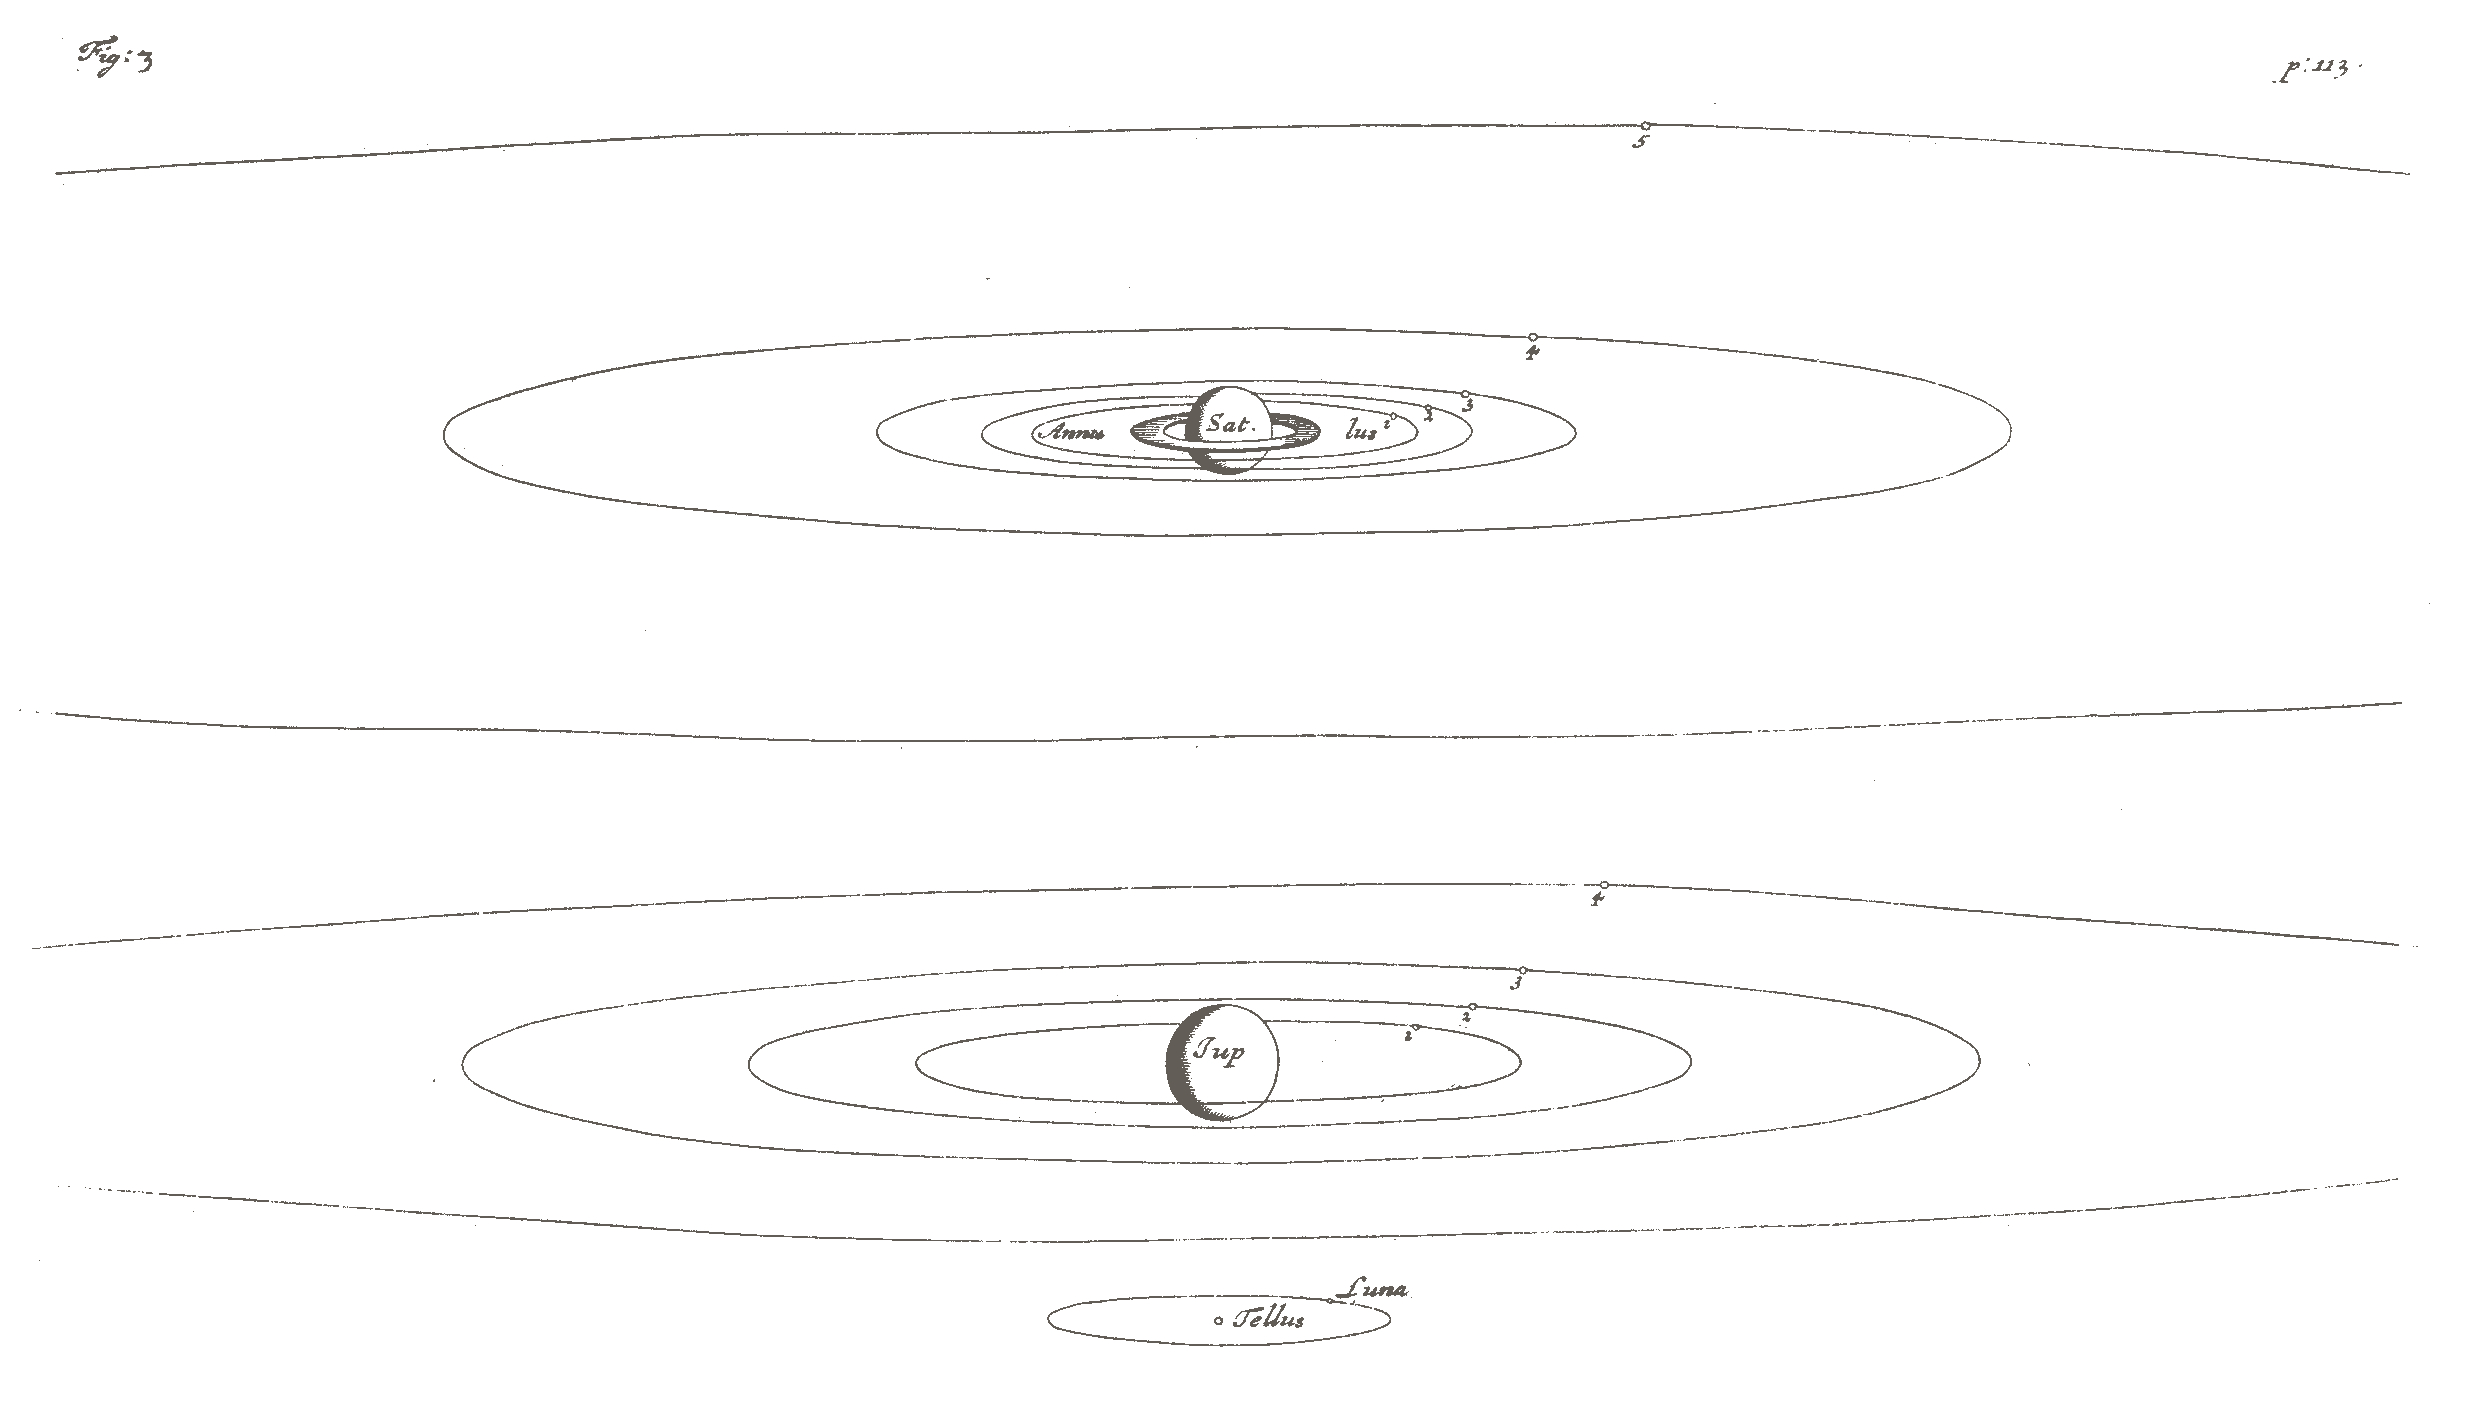
\includegraphics[width=.90\textwidth]{Images/ct_3_en.jpg}
\end{center}

For the eaſier conception of their vaſt diſparity, I have thought
fit [113] to add a Scheme of our Earth, with the Path of the Moon about it,
and the Globe of the Moon it ſelf; and the Syſtems of Jupiter and Saturn,
where I have drawn every thing as near the true Proportion as poſſible.
Jupiter you ſee has his four, and Saturn his five Moons about him, all
plac'd in their Orbits. The Jovial we owe to Galilæo, 'tis well known: and
anyone may imagine he was in no ſmall rapture at the diſcovery. The
outermoſt but one, and brighteſt of Saturn's, it chanc'd to be my lot, with a
Teleſcope not above 12 foot long, to have the firſt ſight of in the year
1655. The reſt we may thank the induſtrious Caſſini for, who uſed the
Glaſſes of Jos.  Campanus's Work, firſt of 36, and afterwards of as many
above 100 foot long. He has often, and particularly in the year 1672, ſhow'd
me the third and fifth. The firſt and ſecond he gave me notice of by Letters
in the year 1684. but they are ſcarce ever to be ſeen, and I can't
poſitively ſay I had ever that happineſs: but am as ſatisfied that they are
[114] there, as if I had; not in the leaſt ſuſpecting the Credit of that
worthy man. Nay, I am afraid there are one or two more ſtill behind, and not
without reaſon. For between the fourth and fifth there's a diſtance not at
all proportionable to that between all the others: Here for ought I know may
lurk a ſixth Gentleman; or perhaps there may be another without the fifth
that may yet have eſcaped us: for we can never ſee the fifth but in that
part of his Orbit, which is towards the Weſt: for which we ſhall give you a
very good reaſon.  Perhaps when Saturn comes into the Northern Signs, and is
at a good height from the Horizon (for at the writing of this he is at his
loweſt) you may happen to make ſome new Diſcoveries, good Brother, if you
would but make uſe of your two Teleſcopes of 170 and 210 foot long; the
longeſt, and the beſt I believe now in the World. For tho we have not yet
had an opportunity of obſerving the Heavens with them (as well by reaſon of
their unweildineſs, as for [115] the interruption of our Studies by your
abſence) yet I am ſatisfied of their Goodneſs by our trial of them one
night, in reading a Letter at a vaſt diſtance by the help of a Light. I
cannot but think of thoſe times with pleaſure, and of our diverting labour
in poliſhing and preparing ſuch Glaſſes, in inventing new Methods and
Engines, and always puſhing forward to ſtill greater and greater things. But
to return to thoſe Diagrams.



\section{The proportion of the Diameter of Jupiter, and of
the Orbs of his Satellites, to the Orbit of the Moon
round the Earth}

I have there made the Diameter of Jupiter about two third parts of our
diſtance from the Moon: for the Diameter of Jupiter is above twenty times
bigger than that of the Earth; which the diſtance of the Moon contains
about thirty times. The Orbit of the outermoſt of Jupiter's Guards is to
that of the Moon round the Earth, as 8 and ? is to 1. And each of theſe
Moons, by the ſhadow they make upon Jupiter, cannot be leſs than our
Earth.


\section{The periods of Jupiter's Moons}

Their Periods, that I may not omit them, are according to Caſſini's account
theſe. That of the inmoſt is one day, 18 hours, 28 minutes, [116] and 36
ſeconds. The ſecond ſpends 3 days, 13 hours, 13 min. 52 ſec. in going
round him. The third 7 days, 3 hours, 59 min. 40 ſec. The fourth 16 days,
18 hours, 5 min. 6 ſec. The diſtance of the innermoſt from Jupiter himſelf
is 2 5/6 of his Diameters. That of the ſecond is 4 and a half: Of the third 7
and one ſixth part: Of the fourth 12 and two thirds, of the ſame Diameters.


\section{And Saturn's}

The innermoſt of Saturn's Guards moves round him in 1 day, 21 hours, 18 min.
31 ſec. The ſecond in 2 days, 17 hours, 41 min. 27 ſec. The third in 4 days,
11 hours, 47 min. 16 ſec. The fourth in 15 days, 22 hours, 41 min. 11 ſec.
The fifth in 79 days, 7 hours, 53 min. 57 ſec. Their diſtances from the
Center of Saturn are, that of the firſt almoſt one, that is 39 fortieth
parts of the Diameter of his Ring; that of the ſecond one and a quarter of
thoſe Diameters; of the third one and three quarters of them; of the fourth
four, or according to my calculation, but 3 and a half; of the fifth 12,
which were found with vaſt pains and labour.  [117] Now can any one took
upon, and compare there Syſtems together, without being amazed at the vaſt
Magnitude and noble Attendance of there two Planets, in reſpect of this
little pitiful Earth of ours? Or can they force themſelves to think, that
the wiſe Creator has diſpoſed of an his Animals and Plants here, has
furniſh'd and adorn'd this Spot only, and has left all thoſe Worlds bare and
deſtitute of Inhabitants, who might adore and worſhip him; or that all thoſe
prodigious Bodies were made only to twinkle to, and be ſtudied by ſome few
perhaps of us poor fellows?


\section{This proportion true according to all modern Obſervations}

I do not doubt but there will be ſome who will think we Romance very
much about the Magnitude of theſe Planets. For will you pretend to make
them who are taken up in admiring the largeneſs of this Globe, its multitude
of Nations, Cities, and Empires; can you pretend I ſay to make them ever
believe that there are Places in compariſon of which the Earth is as inconſiderable as my Figure would make it? No, they know better things [118]
they'l cry. But they may vouchſafe to be inform'd, that theſe Proportions
are thoſe which the beſt Aſtronomers of this Age have agreed upon. For
if the Earth be diſtant from the Sun ten or eleven thouſand of its own Diameters, according to the accounts of Monſieur Caſſini in France, and Mr.
Flamſted in England, wherein they made uſe of very exact Obſervations of
the Parallaxes of Mars; or if, according to a very probable Conjecture of
mine, it be diſtant twelve thouſand, then the Magnitudes of the other Orbs
will very near anſwer the Proportions here ſettled.


\section{The apparent magnitude of the Sun in Jupiter, and a way of finding
what light they there enjoy}

But to return to Jupiter. The Sun appears to them five times leſs than to
us, and conſequently they have but the five and twentieth part of the Light
and Heat that we receive from it. But that Light is not ſo weak there as we
imagine, as is plain by the brightneſs of that Planet in the Night; and that
when the Sun is ſo far eclips'd to us, as that the 25th part of his Disk be
not free from the Shadow, he is not ſenſibly darken'd. But if you have a
[119] mind exactly to know the quantity of light that Jupiter enjoys, you
may take a Tube of what length you pleaſe. Let one end of it be clos'd with a
Plate of Braſs, or any ſuch thing, in the middle of which there muſt be a
hole, whoſe breadth muſt have the ſame proportion to the length of the Tube,
as the Chord of 6 Minutes bears to the Radius; that is about as one is to
570.  Let the Tube be turn'd ſo to the Sun, that no Light may fall upon a
white Paper plac'd at the end of it, but what comes through the little hole
at the other end of the Tube. The Rays that come through this will repreſent
the Sun upon the Paper of the ſame Brightneſs that the Inhabitants of
Jupiter ſee it in a clear day. And if removing the Paper you place your eye
in the ſame place, you will ſee the Sun of the ſame Magnitude and Brightneſs
as you would were you in Jupiter.


\section{And in Saturn}

If you make the hole twice as little in breadth, you will ſee the ſame of
Saturn. And altho his Light be but the hundredth part of ours, yet you
[120] ſee it makes him ſhine finely in a dark night. But in cloudy days what
ſhall the poor Inhabitants do? Why if we were to be Judges but miſerably,
but yet I warrant they do not at all complain. Perhaps they may be like
Owls and Bats, and may love the Twilight better than open day.


\section{In Jupiter their days are 5 hours}

But it's a little ſtrange, that when Jupiter is ſo much bigger than our
Planet, their Days and Nights ſhould be but five of our Hours. By this we
may ſee that Nature has not obſerv'd that proportion that their bulk ſeems
to require, ſeeing in Mars the days are very little different from ours. But
in the length of their years, that is in the revolution of the Planets round
the Sun, there is an exact proportion to their diſtances from the Sun
followed. For as the Cubes of their diſtances, ſo are the Squares of their
Revolutions, as Kepler firſt found out. Which proportion the Moons of
Jupiter and Saturn keep in their Courſes round thoſe.


\section{Always the ſame length}

As the Years and Days in Jupiter are different from ours in this reſpect, ſo
are the Days in another; [121] namely, that they are all of the ſame length.
For they there enjoy a perpetual Equinox, their Axis having little or no
inclination to their Orbit, as the Earth's has, as has bin diſcover'd by
Teleſcopes. The Countries that lie near their Poles have little or no heat,
by reaſon the Rays of the Sun fall ſo obliquely upon them; but then they are
freed from the Inconveniency that ours are troubled with, of tedious long
half-year Nights, and have the conſtant returns of Day and Night every
five hours. Indeed we ſhould not be contented with ſuch ſhort days, and
ſhould count our ſelves very ill dealt with if we had not twice as long, tho
upon no other account, but that what is our own, to be ſure, muſt be beſt.
The reſt of the Planets are ſo near the Sun, (Mars himſelf never being above
18 degrees from it) that in Jupiter they have the ſight only of Saturn.  But
we cannot deny but that their four Moons ſtand them in greater ſtead than
our one doth us, if 'twere only that they ſeldom know any ſuch thing as to
be without Moonſhiny [122] Nights. And they are of great advantage to them,
as we ſaid before, in their Navigation, if they have any ſuch thing. Not to
mention the pleaſant ſights of their frequent Conjunctions and Eclipſes,
things that they are ſeldom a day without.  Saturn enjoys all thoſe
Pleaſures and Advantages in a ſtill higher degree, as well for his five
Moons, as for the delightful proſpect that the Ring about him affords his
Inhabitants night and day. But we will be as kind to them as we have bin to
the reſt of the Planets, in giving an account of their Aſtronomy.


\section{They ſee the fixt Stars juſt as we do}

And firſt of all we ſhall obſerve what we might have remark'd before, but
will be more ſtrange here, that the fix'd Stars appear to them of the ſame
Figure and Magnitude, and with the ſame degree of Light that they do to us:
and this, by reaſon of their immenſe diſtance, of which we ſhall have
occaſion to ſpeak by and by. In compariſon with which the ſpace that a
Bullet ſhot out of a Cannon could travel in 25 years, would be almoſt
nothing.  [123] Their Aſtronomers have all the ſame Signs of the Bear, the
Lion, Orion, and the reſt, but not turning upon the ſame Axis with us: for
that's different in all the Planets.  As Jupiter can ſee no Planet but
Saturn, ſo Saturn knows of no Planet but Jupiter; which appears to him much
as Venus doth to us, never removing above 37 degrees from the Sun. The
length of their days I cannot determine: But if from the diſtance and period
of his innermoſt Attendant, and comparing it with the innermoſt of
Jupiter's, a Man may venture to give a gueſs, they are very little different
from Jupiter's, 10 hours or ſomewhat leſs. But whereas in Jupiter there are
equally divided between Light and Darkneſs, the Saturnians muſt perceive a
more ſenſible difference than we, eſpecially between Summer and Winter. For
our Axis inclines to the place of the Ecliptick but 23 degrees and a half,
but there's above 31. Upon this account his Moons muſt decline very much
from the Path that the Sun ſeems to move [124] in, and his Inhabitants can
never have a full Moon but juſt at the Equinoxes: two of which fall out in
30 of our years. 'Tis this Poſition of the Axis too that is the cauſe of
thoſe delightful appearances, and wonderful proſpects that its Inhabitants
enjoy: for the better underſtanding of which I ſhall draw a Figure of Saturn
with his Ring about him: in which the proportion between the Diameters of
the Globe and Ring is as 9 to 4.  And the empty ſpace between them is of the
ſame breadth with the Ring it ſelf. All Obſervations conſpire to prove that
that is of no great thickneſs, altho if we ſhould allow it ſix hundred
German Miles, I think, conſidering its Diameter, we ſhould not overdo the
matter.  

\begin{center}
	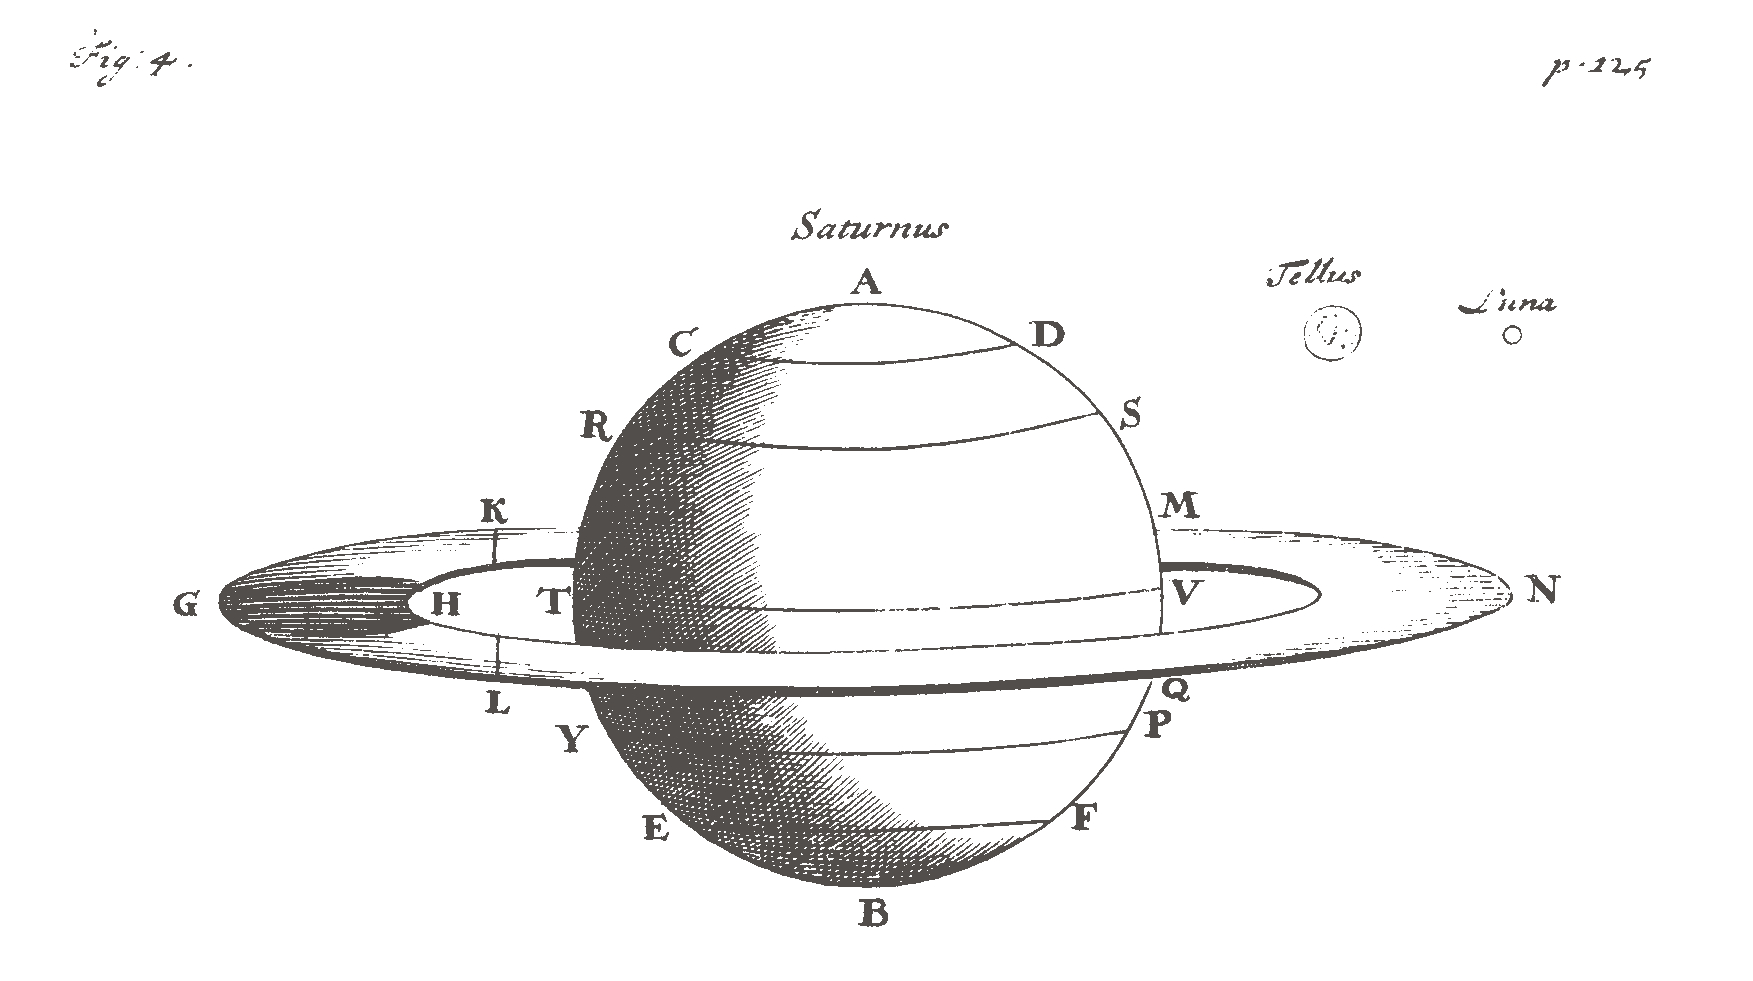
\includegraphics[width=.90\textwidth]{Images/ct_4_en.jpg}
\end{center}

Suppoſe then that to be the Globe of Saturn, whoſe Poles are A, B.
GN es the Diameter of the Ring, as you view it ſideways, repreſenting a
narrow Oval. Thoſe that live about the Poles within the Arches CAD, EBF,
each of which are 54 degrees, (if the Cold will ſuffer any body to live
[125] there) never have a ſight of the Ring.


\section{The appearances of the Ring in Saturn}

From all other parts it is continually to be ſeen for fourteen years and
nine Months, which is juſt: half their year. The other half it is hid from
their view. Thoſe then that dwell between the Polar Circle CD, and the
Equator TV, all that time that the Sun enlightens the part oppoſite to them,
have every night the ſight of a piece of it HGL, much in the ſhape of a
ſhining Bow, which comes from the Horizon, but is darken'd in the middle by
the ſhadow of Saturn GH, which reaches moſt commonly to the outermoſt rim of
it. But after midnight that Shadow by little and little begins to move
towards the right hand to thoſe in the Northern, but the left to thoſe in
the Southern Hemiſphere. In the morning it diſappears, leaving behind it a
likeneſs indeed of a Bow, but much paler and weaker than our Moon is in the
day-time. For they, as I ſaid before, have an Atmoſphere, or an Air
ſurrounding them enlighten'd by the Sun. Otherwiſe Night and Day they would
have their Ring, [126] their Moons, and all the fix'd Stars, equally
conſpicuous. Another thing that muſt make the ſight of their Ring very
curious, is, that by ſome Spots in it, it is diſcover'd to turn round upon
it ſelf: A thing that thoſe that are ſo near cannot but take notice of, when
we that live at this diſtance can deſcry a great Inequality, the inſide of
it being brighter much than the outſide is. When the ſhadow of the Globe
falls upon that part of the Ring GH, the ſhadow of the Ring at the ſame time
darkens another part of the Globe about PF, which otherwiſe would have the
Sun upon it. So that there is always a Zone of the Globe PYFE, ſometimes of a
larger extent than at others, which is depriv'd of the ſight both of the Sun
and Ring for a conſiderable time, the latter of which hides ſome, part of
the Stars from it too. An amazing thing it muſt be, all of a ſudden to have
the Sun darken'd, and, fall into a pitch-night, without ſeeing any cauſe of
ſuch an accident. All which while their Moons are their only Comfort.  The
other half of the [127] year the Hemiſphere TBV enjoys the ſame Light that
TAU before did, and then this undergoes thoſe long Eclipſes that that before
ſuffer'd. At the Equinoxes, when the Sun is in the ſame Plane with the Ring,
the Saturnians cannot well perceive it: no not even we with our Glaſſes, by
reaſon of its Darkneſs. This happens when Saturn, viewed from the Sun, is
advanced one and twenty degrees and a half in Virgo or Piſces, as I ſhow'd
formerly in my Syſtem of Saturn: Where there is an account given of the
Riſings of the Sun above the Ring, throughout all the Saturnian Year.  With
Saturn in this Scheme you have the Globes of the Earth and Moon drawn in
their true proportion, to put you in mind again of a thing very fit to be
remember'd, how very ſmall our Habitation is when compar'd with that Globe
or the Ring about it. And now anyone, I ſuppoſe, can frame to himſelf a
picture of the Night in Saturn, with two Arches of the Ring, and five Moons
ſhining [128] about, and adorning him. This then ſhall be what I have to ſay
to the primary Planets.  We are now come a little lower, to make an enquiry
into the Attendants of there Planets, eſpecially our own. And here we ſhall
meddle not only with their Aſtronomy, but ſhall alſo ſearch into their
Furniture and Ornament, if they are found to have any ſuch thing, which we
have put off conſidering till now.


\section{Very little to be ſaid of the Moon}

And here one would think that when the Moon is ſo near us, and by the
means of a Teleſcope may be ſo nicely and exactly obſerv'd; it ſhould afford us matter for more probable Conjectures than any of the other remote
Planets. But it is quite otherwiſe, and I can ſcarce find any thing to ſay
of it, becauſe I have not a Planet of the ſame nature before my eyes, as in
all the primary ones I have. For they are of the ſame kind with our Earth;
and ſeeing all the Actions, and every thing that is here, we may make a
reaſonable Conjecture at what we cannot ſee in thoſe Worlds.
[129]


\section{The Guards of Jupiter and Saturn of the ſame nature with our Moon}

But this we may venture to ſay, without fear, that all the Attendants of
Jupiter and Saturn are of the ſame nature with our Moon, as going round
them and being carry'd with them round the Sun juſt as the Moon is with
the Earth. Their Likeneſs reaches to other things too, as you'l ſee by and
by. Therefore whatſoever we can with reaſon affirm or fancy of our Moon
(and we may ſay a little of it) muſt be ſuppos'd with very little alteration
to belong to the Guards of Jupiter and Saturn, as having no reaſon to be
at all inferior to that.


\section{The Moon hath Mountains}

The Surface of the Moon then is then found, by the leaſt Teleſcopes of
about three or four foot, to be diverſified with long Tracts of Mountains,
and again with broad Valleys. For in thoſe parts oppoſite to the Sun you
may ſee the Shadows of the Mountains, and often diſcover the little round
Valleys between them, with a hillock or two perhaps riſing out of them.
Kepler from the exact roundneſs of them would prove that they are ſome
vaſt work of the rational [130] Inhabitants. But I can't be of his mind, both
for their incredible largeneſs, and that they might eaſily be occaſion'd by
natural Cauſes.


\section{But no Sea, nor Rivers, nor Clouds, nor Airs and Waters}

Nor can I find any thing like Sea there, tho he and many others are of the
contrary opinion I know. For thoſe vaſt Countries which appear darker than
the other, commonly taken for and call'd by the names of Seas, are diſcver'd
with a good long Teleſcope, to be full of little round Cavities; whoſe
Shadow falling within themſelves, makes them appear of that colour: and
thoſe large Champains there in the Moon you will find not to be always even
and ſmooth, if you look carefully upon them: neither of which two things can
agree to the Sea. Therefore thoſe Plains in her that ſeem brighter than the
other parts, muſt conſiſt, I ſuppoſe, of a whiter ſort of Matter than they.
Nor do I believe that there are any Rivers, for if there were, they could
never eſcape our ſight, eſpecially if they run between the Hills as ours
do.  Nor have they any Clouds to furniſh the Rivers with [131] Water. For if
they had, we ſhould ſometimes ſee one part of the Moon darken'd by them, and
ſometimes another, whereas we have always the ſame proſpect of her.  'Tis
certain moreover, that the Moon has no Air or Atmoſphere ſurrounding it as
we have. For then we could never ſee the very outermoſt Rim of the Moon ſo
exactly as we do, when any Star goes under it, but its Light would terminate
in a gradual faint ſhade, and there would be a ſort of a down as it were
about it; not to mention, that the Vapors of our Atmoſphere conſiſt of
Water, and conſequently that where there are no Seas or Rivers, there can be
no Atmoſphere. This is that notable difference between that Planet and us
that hinders all probable Conjectures about it. If we could but once be ſure
that they had Water, we might come to an Agreement, and plant a Colony
perhaps there; we might allow it then moſt of our other Privileges, and,
with Xenophanes, furniſh it with Inhabitants, Cities, and Mountains. But as
'tis, I [132] cannot imagine how any Plants or Animals, whoſe whole
nouriſhment comes from liquid Bodies, can thrive in a dry, waterleſs,
parch'd Soil.


\section{The Conjecture of its Plants and Animals very dubious}

What then, ſhall this great Ball be made for, nothing but to give us a little
puny light in the Night-time, or to raiſe our Tides in the Sea? Shall not
we plant ſome People there that may have the pleaſure of ſeeing our Earth
turn upon itſelf, preſenting them ſome times with a proſpect of Europe and
Africa, and then of Aſia and America; ſometimes half, and ſometimes full?
What! and muſt all thoſe Moons round Jupiter and Saturn be condemn'd
to the ſame uſeleſneſs? I do not know what to think of it, becauſe I know
of nothing like them to found a Conjecture upon. And yet 'tis not improbable that thoſe great and noble Bodies have ſomewhat or other growing
and living upon them, tho very different from what we ſee and enjoy here.
Perhaps their Plants and Animals may have another ſort of Nouriſhment
there. Perhaps the moiſture of the Earth there is but juſt ſufficient [133]
to cauſe a Miſt or Dew, which may be very ſutable to the growth of their
Herbs. Which I remember is Plutarch's opinion, in his Dialogue upon this
Subject. For in our Earth a very little Water drawn from the Sea into Dew,
and falling down again upon the Herbs, would be ſufficient for all our needs,
without any Rain or Showers.


\section{Jupiter's and Saturn's Moons turn always the ſame ſide to them}

But theſe are mere gueſſes, or rather doubts, but yet they are the beſt we
can make of this, and all thoſe other Moons: for, as I ſaid before, they are
all of the ſame nature, which is proved likewiſe by this, that as our Moon
can afford us the ſight never but of one ſide of her, ſo they turn always
the ſame face to their primary Planets. You wonder, I ſuppoſe, how we came
to know ſo much; but 'twas no hard matter, after that Obſervation which I
juſt now made, that the outermoſt of Saturn's Moons can never be ſeen but
when ſhe is on the Weſt-ſide of her Planet. The reaſon of which is plainly
this, that one ſide of her is darker, and does not reflect the Light ſo much
as the other, [134] which when it is turned towards us, we cannot ſee by
reaſon of its weak Light. This always happening when 'tis Eaſt of him, and
never on the other ſide, is a manifeſt proof that ſhe always keeps the ſame
ſide toward Saturn. Now ſince the outermoſt of Saturn's and our Moon carry
themſelves thus to the Planets round which they move, who can well doubt it
of all the reſt round Jupiter and Saturn? And there's a very good reaſon for
it, namely, that the matter of which thoſe Moons conſiſt, being heavier, and
more ſolid on the ſide that is averſe from us, than on that which we have
the ſight of, does conſequently fly with a greater force from the Centre of
its Motion: for otherwiſe, according to the Laws of Motion, it ſhould turn
the ſame ſide always, not to its Planet; but to the ſame fixt Stars.  This
Poſition of the Moons, in reſpect of their Planets, muſt occaſion great many
very pretty, wonderful ſights to their Inhabitants, if they have any: which
is very doubtful, but may for the preſent be ſuppos'd.  [135]


\section{The Aſtronomy of the Inhabitants of the Moon}

An enquiry into our Moon may ſerve for all the reſt. Its Globe is divided
into two parts, after that manner, that thoſe who live on one ſide never
loſe the ſight of us, and thoſe on the other never enjoy it. Only thoſe who
live on the Confines of each of theſe loſe us, and ſee us again by turns. The
Earth to them muſt ſeem much larger than the Moon doth to us, as being in
Diameter above four times bigger. But the beſt of it is, that night and day
they ſee it always in the very ſame part of the Heaven, as if it never moved:
ſome of them as if 'twas falling upon their heads: others ſomewhat above
the Horizon, and others always in the Horizon, ſtill turning upon it ſelf, and
preſenting them every twenty four hours with a view of all its Countries,
even of thoſe that lie near the Poles (I could wiſh my ſelf in the Moon only
for the ſight of them) yet unknown and undiſcover'd by us. They have it
in its monthly Wane and Increaſe, they ſee it half, and horned, and full, by
turns, juſt as we do their Planet. But the Light [136] that they borrow of us
is five times larger than what they pay us again. So that in dark nights that
part that hath the advantage of being towards us, receives a very glorious
Light, tho let Kepler ſay what he will, no Heat from us. Their Days are
always of the ſame length with their Nights; and the Sun riſing and ſetting
to them but once in one of our Months, makes the time both of their Light
and Darkneſs to be equal to 15 of our days. If their Bodies are of the ſame
Metal with ours, thoſe that have the Sun pretty high in their Horizon, muſt
be like to be burnt up in ſuch long days. For the Sun is not farther from
them than he is from us. This will be the caſe of thoſe that live upon the
Borders of the two Hemiſpheres we talk'd of; but thoſe that live under the
Poles of the Moon will be juſt about as hot as our Whale-Fiſhers about
Iſland and Nova Zemla are, in the Summer-time: who are in ſo little danger
of being roaſted, that in the middle of their Summer, in their days of three
Months length, they are ready to loſe their [137] fingers ends. The Poles
of the Moon I call thoſe, round which the fixt Stars ſeem to turn to its
Inhabitants, which are different from ours, and thoſe of the Ecliptick, altho
they move round theſe latter, at the diſtance of five degrees, in a period
of nineteen Years. Their Year they count by the Motion of the Stars, and
their return to the Sun, and 'tis the ſame with ours. They can eaſily do it,
becauſe they have the Stars day and night, notwithſtanding the Light of the
Sun: for they have no Atmoſphere (which is the only reaſon that we don't
every day enjoy the ſame ſight) to hinder their Obſervations. Nor have
they any Clouds to obſtruct their view, ſo that they have an eaſier work
than we to find out the Courſes, but a more difficult to make a true Syſtem
of the Planets. For they will be apt to lay a wrong Foundation upon the
Immobility of the Earth, which will lead them into more dangerous Errors
than ever it did us.


\section{This may be applied to the Moons about Jupiter and Saturn}

All that I have ſaid belongs as well to Jupiter's and Saturn's as to our Moon
in reſpect of [138] the Planets they move round. The length of their Day and
Night is always equal to the time of their Revolution: for example, the fifth
Moon moves round Saturn in 80 days, and the days and nights there are equal to
forty of ours. Both their Summer and Winter (Saturn moving round the Sun in
thirty years) are fifteen years long. Therefore it is impoſſible but that their
way of living muſt be very different from ours, having ſuch tedious Winters,
and ſuch long watching and ſleeping times.  Having thus explain'd the primary
and ſecondary Planets round the Sun, we ſhould next ſet about the third ſort,
the Sun and fixt Stars; but before we do that, it will be worth while to ſet
before you at once, in a clearer and more plain Method than hitherto, the
Magnificence and Fabrick of the Solar Syſtem. Which we can't poſſibly do in ſo
ſmall a ſpace as one of our Leaves will but admit of, becauſe the Bodies of the
Planets are ſo prodigiouſly ſmall in compariſon of their Orbs. But what is
wanting in Figure ſhall be [139] made up in Words. Going back then to the firſt
Scheme, ſuppoſe another like it, and proportionable, drawn upon a very large
ſmooth Plain; whoſe outermoſt Circle repreſenting the Orb of Saturn, muſt be
conceived three hundred and ſixty foot in Semi-diameter. In which you muſt
place the Globe and Ring of Saturn of that bigneſs as the 2d Figure ſhows you.
Let all the other Planets be ſuppoſed everyone in his own Orbit, and in the
middle of all the Sun, of the ſame bigneſs that that Figure repreſents, namely,
about four inches in Diameter. And then the Orbit or Circle in which the Earth
moves, which the Aſtronomers call the magnus Orbis, muſt have about ſix and
thirty foot in Semidiameter. In which the Earth muſt be conceived moving, not
bigger than a grain of Millet, and her Companion the Moon ſcarcely perceivable,
moving round her in a Circle a little more than two Inches broad, as in the
Figure here adjoined, where the line AB repreſents a ſmall portion of that
Circle which the Earth moves in: [140] the ſmall Circle therein C is the Earth
and the Circle DE the path of the Moon round it, in which the body of the Moon
is D.  

\begin{center}
	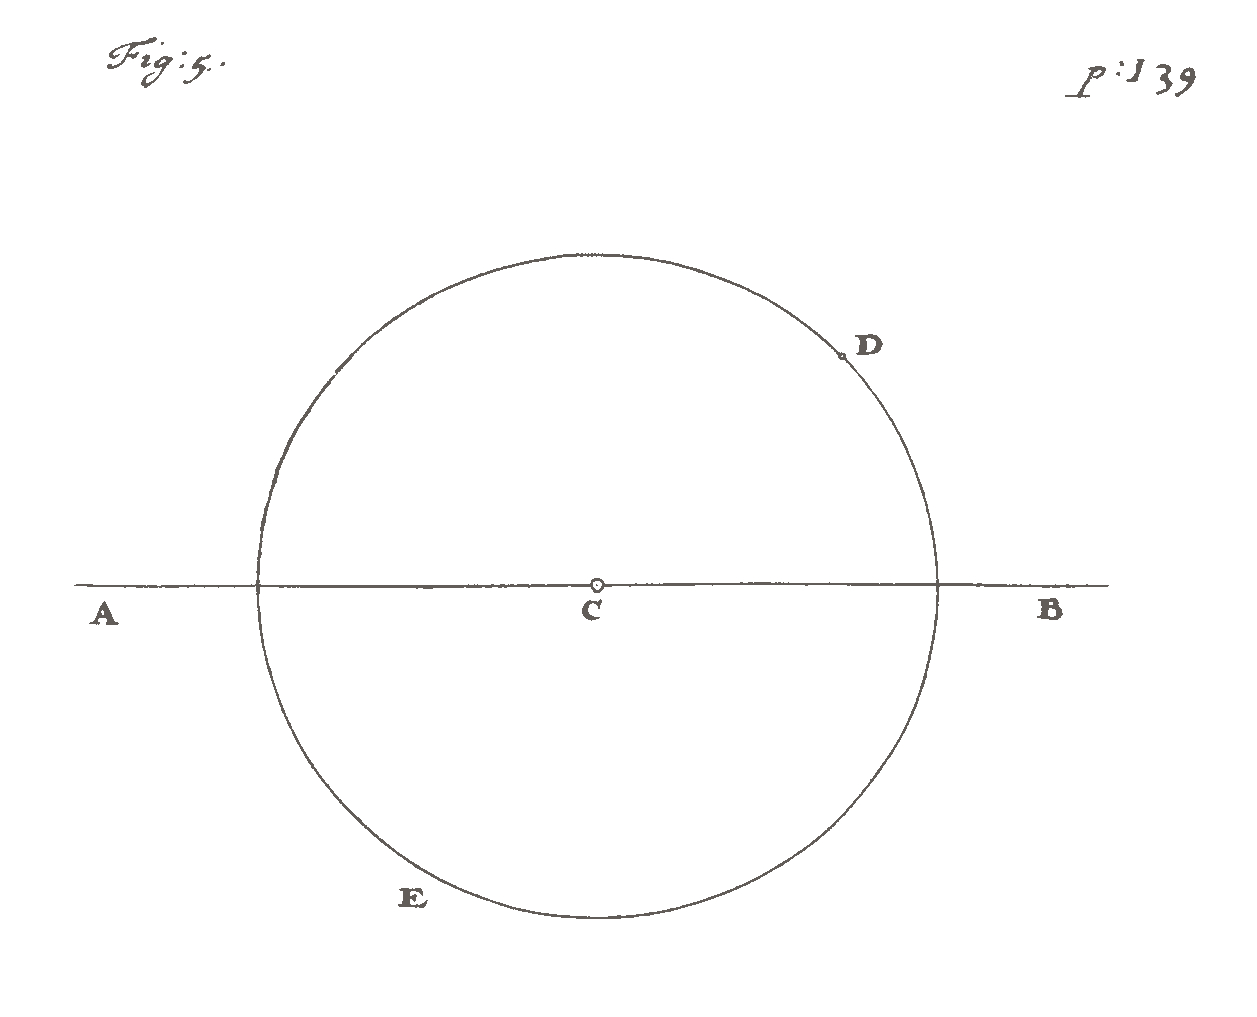
\includegraphics[width=.90\textwidth]{Images/ct_5_en.jpg}
\end{center}

The outermoſt of Saturn's Moons move in an Orbit whoſe Semidiameter is
29 inches; that of Jupiter in a ſomewhat ſmaller, whoſe Semidiameter is 19 and
a quarter.  And thus we have a true and exact Deſcription of the Sun's Palace,
where the Earth will be twelve thouſand of its Semidiameters diſtant from him,
which in German Miles makes above ſeventeen Millions. But perhaps we may have a
clearer comprehenſion of this vaſt length, by comparing it with ſome very ſwift
Motion. 'Twas a pretty fancy of Heſiod, that an Anvil let fall from the top of
Heaven, reach'd the Earth the tenth day of its Journey, and in ten more arriv'd
at the bottom of Hell, the end of it: ſo making the Earth the midway between
Heaven and Hell. I ſhan't make uſe of the Anvil, but of one as good, namely, a
Bullet ſhot out of a great Gun, which may travel per[141]haps in a moment, or
pulſe of an Artery, about a hundred Fathom, as is prov'd by thoſe Experiments
that Merſennnus in a Treatiſe of his relates; wherein the Sound was found to
extend it ſelf eighty hundredth parts in that time.


\section{The immenſe diſtance between the Sun and the Planets illuſtrated}

I ſay then, that ſuppoſing a Bullet to move with this ſwiftneſs from the
Earth to the Sun, it would ſpend 25 years in its paſſage. To make a Journey
from Jupiter to the Sun, would require 125, and from Saturn thither 250
years. This account depends upon the meaſure of the Earth's Diameter,
which, according to the accurate Obſervations of the French, is 6 538 594
times ſix Paris feet, one degree being 57 060 of that meaſure. This ſhows
us how vaſt thoſe Orbs muſt be, and how inconſiderable this Earth, the
Theatre upon which all our mighty Deſigns, all our Navigations, and all our
Wars are tranſacted, is when compared to them. A very fit Conſideration,
and matter of Reflection, for thoſe Kings and Princes who ſacrifice the Lives
of ſo many People, only to flatter their Ambition in being [142] Maſters of
ſome pitiful corner of this ſmall Spot. But to return to the matter in hand,
now we have given you an account of the Sun's proportion to thoſe Orbs
and Bodies, we'll ſee what more we can ſay of him.


\section{No ground for Conjecture in the Sun}

And there are ſome that have bin ſo civil, as to allow the Sun himſelf his
Inhabitants. But upon what reaſon I cannot imagine, there being leſs
ground for a probability in him than in the Moon. For we are not yet ſure,
whether he be a compact or liquid Globe; altho, if my account of Light be
true, upon that account I ſhould rather think him liquid: which his
roundneſs and equal diſtribution of his Light to all parts are an Argument
for. For that inequality on his Surface, which is diſcover'd by the
Teleſcopes, (and that not always neither) which makes men fancy boiling Seas
and belching Mountains of Fire, is nothing but the trembling Motion of the
Vapors our Atmoſphere is full of near the Earth; which is likewiſe the cauſe
of the Stars twinkling.


\section{The Faculæ in the Sun not eaſily ſeen}

Nor could I ever have the luck to diſcern thoſe [143] bright Spots they brag
ſo much of in the Sun as well as of his dark ones, tho the latter I have very
often ſeen; ſo that with very good reaſon I can doubt whether there's any
ſuch thing. For, in all the exact Obſervations, I could never find any ſuch
pretended to be ſeen any where but juſt about his dark Spots; and it is no
great wonder that thoſe Parts which are ſo near the darker, ſhould appear
ſomewhat brighter than the reſt.


\section{By reaſon of its Heat no Inhabitants like ours can live in the Sun}

That the Sun is extremely hot and firy, is beyond all diſpute, and ſuch
Bodies as ours could not live one moment in ſuch a Furnace. We muſt make new
ſort of Animals then, ſuch as we have no Idea or Likeneſs of among us, ſuch
as we can neither imagine nor conceive: which is as much as to ſay, that
truly we have nothing at all to ſay. No doubt that glorious and vaſt Body
was made for ſome noble end and uſe, and fram'd with excellent deſign.  And I
think we all very well know and feel its Uſefulneſs in that effuſion of
Light and Heat to all the Planets round it; in the preſervation and
happineſs of all [144] living Creatures, and that not only in our Ball, but
in thoſe vaſt Globes of Jupiter and Saturn, not much inferior to its own.
Theſe are ſuch great, ſuch wiſe ends, that it is not ſtrange that the Sun
ſhould have bin made, if it had bin only upon their account. For, as for
Kepler's fancy, that he hath another Office, namely, to help on the Motion
of the Planets in their own Orbs, by turning them round their Axis, (which
he would fain eſtabliſh in his Epitome) I ſhall give good Reaſons why I
cannot aſſent to it.


\section{The fix'd Stars ſo many Suns}

Before the invention of Teleſcopes, Stars ſo it ſeem'd to contradict Copernicus's Opinion, to make the Sun one of the fix'd Stars. For the Stars of
the firſt Magnitude being eſteemed to be about three minutes Diameter; and
Copernicus (obſerving that tho the Earth changed its place, they always kept
the ſame diſtance from us) having ventur'd to ſay that the Magnus Orbis was
but a point in reſpect of the Sphere in which they were placed, it was a
plain conſequence that everyone of them that appeared any thing bright, muſt
[145] be larger than the Path or Orbit of the Earth: which is very abſurd.
This is the topping Argument that Tycho Brahe ſet up againſt Copernicus. But
when the Teleſcopes ſhav'd them of their fictitious Rays, and ſhow'd 'em to
us bare and naked (which they do beſt when the Eye-glaſs is black'd with
Smoke) juſt like little ſhining Points, then that difficulty vaniſhed, and
the Stars might ſtill be Suns. Which is the more probable, becauſe their
Light is certainly their own: for it's impoſſible that ever the Sun ſhould
ſend, or they reflect it at ſuch a vaſt diſtance. This is the opinion that
commonly goes along with Copernicus's Syſtem.


\section{They are not all in the ſame Sphere}

And the Patrons of it do alſo with reaſon ſuppoſe, that all theſe Stars are
not in the ſame Sphere, as well becauſe there's no Argument for it, as that
the Sun, which is one of them, cannot be brought to this Rule. But it's
more likely they are ſcatter'd and diſperſed all over the immenſe ſpaces of
the Heaven, and are as far diſtant perhaps from one another, as the neareſt
of them are from the Sun.
[146] Here again too I know Kepler is of another opinion in his Epitome
of Copernicus's Syſtem, that we mention'd above. For tho he agrees with
us, that the Stars are diffus'd through all the vaſt Profundity, yet he cannot
allow that they have as large an empty ſpace about them as our Sun has.
For at that rate, 'twas his opinion, we ſhould ſee but very few, and thoſe of
very different Magnitudes: For, ſeeing the largeſt of all appear ſo ſmall to
us, that we can ſcarce obſerve or meaſure them with our beſt Inſtruments;
how muſt thoſe appear that are three or four times farther from us? Why,
ſuppoſing them no larger than theſe, they muſt ſeem three or four times
leſs, and ſo on till a little farther they will not be to be ſeen at all: Thus we
ſhall have the ſight of but very few Stars, and thoſe very different one from
another; Whereas we have thouſands, and thoſe not conſiderably bigger or
leſs than one another. But this by no means proves what he would have
it; and his miſtake was chiefly, that he did not conſider the nature of Fire,
which makes it be ſeen at ſuch [147] diſtances, and at ſuch ſmall Angles as
all other Bodies would totally diſappear under. A thing that we need go no
farther than the Lamps ſet along the Streets to prove. For altho they are
a hundred foot from one another, yet you may count twenty of them in a
continued row with your eyes, and yet the twentieth of them ſcarce makes
an Angle of ſix Seconds. Certainly then the glorious Light of the Stars muſt
do much more than this; ſo that it's no wonder we ſhould ſee a thouſand
or two of them with our bare eyes, and with a Teleſcope diſcover twenty
times that number. But Kepler had a private deſign in making the Sun
thus ſuperior to all the other Stars, and planting it in the middle of the
World, attended with the Planets: a favor that he did not deſire to grant
the reſt. For his aim was by it to ſtrengthen his Coſmographical Myſtery,
that the diſtances of the Planets from the Sun are in a certain proportion
to the Diameters of the Spheres that are inſcrib'd within, and circumſcrib'd
about Euclid's Polyedrical Bodies. [148] Which could never be ſo much as
probable, except there were but one Chorus of Planets moving round the
Sun, and ſo the Sun were the only one of his kind.
But that whole Myſtery is nothing but an idle Dream taken from Pythagoras or Plato's Philoſophy. And the Author himſelf acknowleges that the
Proportions do not agree ſo well as they ſhould, and is fain to invent two or
three very ſilly excuſes for it. And he uſes yet poorer Arguments to prove
that the Univerſe is of a ſpherical Figure, and that the number of the Stars
muſt neceſſarily be finite, becauſe the Magnitude of each of them is ſo.
But what is worſt of all is, that he ſettles the ſpace between the Sun and
the concavity of the Sphere of the fix'd Stars, to be ſix hundred thouſand
of the Earth's Diameters. For this very good reaſon, forſooth, that as the
Diameter of the Sun is to that of the Orbit of Saturn, which he makes to be
as 1 to 2000, ſo is this Diameter to that of the Sphere of the fix'd Stars. A
mere fancy without any ſhadow of [149] Reaſon. I cannot but wonder how
ſuch things as theſe could fall from ſo ingenious a Man, and ſo great an
Aſtronomer. But I muſt give my Vote, with all the greateſt Philoſophers of
our Age, to have the Sun of the ſame nature with the fix'd Stars. And this
will give us a greater Idea of the World, than all thoſe other Opinions.


\section{The Stars have Planets about them like our Sun}

For then why may not every one of theſe Stars or Suns have as great a
Retinue as our Sun, of Planets, with their Moons, to wait upon them? Nay
there's a manifeſt reaſon why they ſhould. For let us fancy our ſelves
placed at an equal diſtance from the Sun and fix'd Stars; we ſhould then
perceive no difference between them. For, as for all the Planets that we now
ſee attend the Sun, we ſhould not have the leaſt glimpſe of them, either
that their Light would be too weak to affect us, or that all the Orbs in
which they move would make up one lucid point with the Sun. In this ſtation
we ſhould have no occaſion to imagine any difference between the Stars, and
ſhould make no doubt if we [150] had but the ſight, and knew the nature of
one of them, to make that the Standard of all the reſt. We are then plac'd
near one of them, namely, our Sun, and ſo near as to diſcover ſix other
Globes moving round him, ſome of them having others performing them the ſame
Office.  Why then ſhall not we make uſe of the ſame Judgment that we would
in that caſe; and conclude, that our Star has no better attendance than the
others?  So that what we allow'd the Planets, upon the account of our
enjoying it, we muſt likewiſe grant to all thoſe Planets that ſurround that
prodigious number of Suns. They muſt have their Plants and Animals, nay and
their rational ones too, and thoſe as great Admirers, and as diligent
Obſervers of the Heavens as our ſelves; and muſt conſequently enjoy
whatſoever is ſubſervient to, and requiſit for ſuch Knowlege.  What a
wonderful and amazing Scheme have we here of the magnificent Vaſtneſs of the
Univerſe! So many Suns, ſo many Earths, and every one of them ſtock'd with
ſo many [151] Herbs, Trees and Animals, and adorn'd with ſo many Seas and
Mountains! And how muſt our wonder and admiration be encreaſed when we
conſider the prodigious diſtance and multitude of the Stars?  That their
diſtance is ſo immenſe, that the ſpace between the Earth and Sun (which is
no leſs than twelve thouſand of the former's Diameters) is almoſt nothing
when compar'd to it, has more Proofs than one to confirm it. And this among
the reſt, If you obſerve two Stars near one another, as for example thoſe in
the middle of the Great Bears Tail, differing very much from one another in
Clearneſs, notwithſtanding our changing our Poſition in our Annual Orbit
round the Sun, and that there would be a Parallax were the Star which is
brighter nearer us than the other, as is very probable it is, yet whatever
part of the year you look upon them, they will not in the leaſt have altered
their diſtance. Thoſe that have hitherto undertook to calculate their
Diſtance, have not bin able perfectly to [152] compaſs their deſign, by
reaſon of the extreme niceneſs and almoſt impoſſibility of the Obſervations
requiſite for their purpoſe. The only Method that I ſee remaining, to come
at any tolerable probability in ſo difficult a caſe, I ſhall here make uſe
of. Seeing then that the Stars, as I ſaid before, are ſo many Suns, if we do
but ſuppoſe one of them equal to ours, it will follow that its diſtance from
us is as much greater than that of the Sun, as its apparent Diameter is leſs
than the Diameter of the Sun. But the Stars, even thoſe of the firſt:
Magnitude, tho view'd through a Teleſcope, are ſo very ſmall that they ſeem
only like ſo many ſhining Points, without any perceivable breadth. So that
ſuch Obſervations can here do us no good.


\section{A way of making a probable gueſs at the diſtance of the Stars}

When I ſaw this would not ſucceed, I ſtudied by what way I could ſo leſſen
the Diameter of the Sun, as to make it not appear larger than the Dog,
or any, other of the chief ſtars. To this purpoſe I clos'd one end of my
twelve-foot Tube with a very thin Plate, in the middle of which I made a
hole not [153] exceeding the twelfth part of a Line, that is the hundred and
forty fourth part of an Inch. That end I turn'd to the Sun, placing my Eye
at the other, and I could ſee ſo much of the Sun as was in Diameter about
the 182d part of the whole. But ſtill that little piece of him was brighter
much than the Dog-Star is in the cleareſt night. I ſaw that this would not
do, but that I muſt leſſen the Diameter of the Sun a great deal more. I
made then ſuch another hole in a Plate, and againſt it I plac'd a little round
Glaſs that I had made uſe of in my Microſcopes, of much about the ſame
Diameter with the former hole. Then looking again towards the Sun (taking
care that no Light might come near my eye to hinder my Obſervation) I
found it appear'd of much the ſame Clearneſs with Sirius. But caſting up
my account, according to the Rules of Dioptricks, I found his Diameter now
was but 1/152 part of that hundred and eighty ſecond part of his whole
Diameter that I ſaw through the former hole. Multiplying 1/152 and 1/182
into [154] one another, the Product I found to be 1/27664. The Sun therefore
being contracted into ſuch a compaſs, or being removed ſo far from us (for
it's the ſame thing) as to make his Diameter but the 27664 part of that we
every day ſee, will ſend us ſtill the ſame Light as the Dog-ſtar now doth.
And his diſtance then from us will be to his preſent diſtance undoubtedly
as 27664 is to 1; and his Diameter little above four thirds, 4”'. Seeing then
Sirius is ſuppoſed equal to the Sun, it follows that his Diameter is likewiſe
4”', and that his diſtance to the diſtance of the Sun from us is as 27664 to
1. And what an incredible diſtance that is, will appear by the ſame way of
reaſoning that we uſed in meaſuring that of the Sun. For if 25 years are
required for a Bullet out of a Cannon, with its utmoſt Swiftneſs, to travel
from the Sun to us; then by multiplying the number 27664 into 25, we ſhall
find that ſuch a Bullet would ſpend almoſt ſeven hundred thouſand years
in its Journey between us and the neareſt of the fix'd [155] Stars. And yet
when in a clear night we look upon them, we cannot think them above ſome
few miles over our heads. What I have here enquir'd into, is concerning
the neareſt of them, And what a prodigious number muſt there be beſides
of thoſe which are, placed ſo deep, in the vaſt ſpaces of Heaven, as to be
as remote from there as there are from the Sun! For if with our bare Eye
we can obſerve above a thouſand, and with a Teleſcope can diſcover ten or
twenty times as many; what bounds of number muſt we ſet to thoſe which
are out of the reach even of theſe Aſſiſtances! eſpecially if we confider
the infinite Power of God. Really, when I have bin reflecting thus with my
ſelf, methoughts all our Arithmetick was nothing, and we are vers'd but
in the very Rudiments of Numbers, in compariſon of this great Sum. For
this requires an immenſe Treaſury, not of twenty or thirty Figures only, in
our decuple Progreſſion, but of as many as there are Grains of Sand upon
the ſhore. And yet who can ſay, that [156] even this number exceeds that
of the Fixt Stars? Some of the Antients, and Jordanus Brunus carry'd it
further, in declaring the Number infinite: he would perſwade us that he has
prov'd it by many Arguments, tho in my opinion they are none of them
concluſive. Not that I think the contrary can ever be made out. Indeed it
ſeems to me certain, that the Univerſe is infinitely extended; but what God
has bin pleas'd to place beyond the Region of the Stars, is as much above
our Knowlege, as it is our Habitation.
Or what if beyond ſuch a determinate ſpace he has left an infinite Vacuum; to ſhow, how inconſiderable all that he has made is, to what his Power
could, had he ſo pleas'd, have produc'd? But I am falling, before I am aware,
into that intricate Diſpute of Infinity: Therefore I ſhall wave this, and not,
as ſoon as I am free of one, take upon me another difficult Task. All that I
ſhall do more is to add ſomewhat of my opinion concerning the World, as
it is a place for the reception of the Suns or fix'd Stars, [157] every one of
which, I have ſhow'd may have their Planetary Syſtems about them.


\section{Every Sun has a Vortex round it, very different from thoſe of Cartes}

I am of opinion then that every Sun is ſurrounded with a Whirl-pool or
Vortex of Matter in a very ſwift Motion; tho not in the leaſt like Cartes's
either in their bulk, or manner of Motion. For Cartes makes his ſo large,
as everyone of them to touch all the others round them, in a flat Surface,
juſt as you have ſeen the Bladders that Boys blow up in Soap-ſuds do: and
would have the whole Vortex to move round the ſame way. But the Angles
of every Vortex will be no ſmall hindrance to ſuch a Motion. Then the whole
matter moving round at once, upon the Axis as it were of a Cylinder, did not
a little puzzle him in giving Reaſons for the Roundneſs of the Sun: which
however they may ſatisfy ſome People that do not conſider them, really
prove nothing of the matter. In this æthereal matter the Planets float, and
are carry'd round by its motion: and the thing that keeps them in their own
Orbs is, that they [158] themſelves, and the matter in which they ſwim.
equally ſtrive to fly out from the Center of this Motion. Againſt all which
there are many Aſtronomical Objections, ſome of which I touch'd upon in
my Eſſay of the Cauſes of Gravity. Where I gave another account of the
Planets not deſerting their own Orbs; which is their Gravitation towards
the Sun. I ſhow'd there the Cauſes of that Gravitation, and cannot but
wonder that Cartes, the firſt man that ever began to talk reaſonably of that
matter, ſhould never meddle with, or light on it. Plutarch in his Book of
the Moon above mentioned ſays, that ſome of the Antients were of opinion,
that the reaſon of the Moon's keeping her Orbit was, that the force of her
Circular Motion was exactly equal to her Gravity, the one of which pull'd
her to, as much as the Other forc'd her off from the Centre. And in our
Age Alphonſus Borellus, who was of this ſame opinion in the other Planets
as well as the Moon, makes the Gravitation of the primary Planets to be
towards the Sun, as that of the ſecondary is towards the Planets round
which they move: Which Mr. Iſaac Newton has more fully explained, with
a great deal of pains and ſubtilty; and how from that cauſe proceeds the
Ellipticity of the Orbs of the Planets, found out by Kepler. According to
my Notion of the Gra[159]vitation of the Planets to the Sun, the matter of
his Vortex muſt not all move the ſame way, but after ſuch a manner as to
have its parts carry'd different ways on all ſides. And yet there is no fear of
its being deſtroy'd by ſuch an irregular motion, becauſe the Æther round it,
which is at reſt, keeps the parts of it from flying out. With the help of ſuch
a Vortex as this I have pretended in that Eſſay to explain the Gravity of
Bodies on this Earth, and all the effects of it. And I ſuppoſe there may be
the ſame cauſe as well of the Gravitation of the Planers, and of our Earth
among the reſt, towards the Sun, as of their Roundneſs: a thing ſo very
hard to give an account of in Cartes's Syſtem.
I muſt differ from him too in the bigneſs of the Vortices, for I cannot allow
them to be ſo large as he would make them. I would have them diſpers'd
all about the immenſe ſpace, like ſo many little Whirl-pools of Water, that
one makes by the ſtirring of a ſtick in any large Pond or River, a great
way diſtant from one another. And as their motions do not all intermix or
communicate with one another; ſo in my opinion muſt the Vortices of Stars
be plac'd as not to hinder one anothers free Circumrotations.
So that we may be ſecure, and never fear that they will ſwallow up or
deſtroy one another; for that was a mere fancy of Car[160]tes's; when he
was ſhowing how a fix'd Star or Sun might be turn'd into a Planet. And 'tis
plain, that when he writ it, he had no thoughts of the immenſe diſtance of
the Stars from one another; particularly, by this one thing, that he would
have a Comet as ſoon as ever it comes into our Vortex, to be ſeen by us.
Which is as abſurd as can be. For how could a Star, which gives us ſuch a
vaſt Light only from the Reflection of the Beams of the Sun, as he himſelf
owns they do; how I ſay could that be ſo plainly ſeen at a diſtance ten
thouſand times larger than the Diameter of the Earth's Orbit? He could
not but know that all round the Sun there is a vaſt Extenſum; ſo vaſt,
that in Copernicus's Syſtem the magnus Orbis is counted but a point in
compariſon with it. But indeed all the whole ſtory of Comets and Planets,
and the Production of the World, is founded upon ſuch poor and trifling
grounds, that I have often wonder'd how an ingenious man could ſpend all
that pains in making ſuch fancies hang together. For my part, I ſhall be
very well contented, and ſhall count I have done a great matter, if I can
but come to any knowlege of the nature of things, as they now are, never
troubling my head about their beginning, or how they were made, knowing
that to be out of the reach of human Knowlege, or even Conjecture.

\em{FINIS}
\end{document}
